\documentclass[lettersize,journal]{IEEEtran}
\usepackage{amsmath,amsfonts}
\usepackage{algorithmic}
\usepackage{algorithm}
\usepackage{array}
\usepackage[caption=false,font=normalsize,labelfont=sf,textfont=sf]{subfig}
\usepackage{textcomp}
\usepackage{stfloats}
\usepackage{url}
\usepackage{verbatim}
\usepackage{graphicx}
\usepackage{cite}
\hyphenation{op-tical net-works semi-conduc-tor IEEE-Xplore}
% updated with editorial comments 8/9/2021
\usepackage{booktabs}
\usepackage{multirow}
\usepackage{microtype}
\usepackage[utf8]{inputenc}
\usepackage{comment}
\usepackage[table]{xcolor}
\newcommand{\revise}[1]{\textcolor{blue}{#1}}
\begin{document}

\title{DDBR: Personalized Discrete Diffusion Model for Cold-start Bundle Recommendation}

\author{Zhijing Yang,
        Jin Wang,
        and~Jinghui Qin         
        % <-this % stops a space
\thanks{
Zhijing Yang, Jin Wang, and Jinghui Qin are with the School of Information Engineering, Guangdong University of Technology. (email:  yzhj@gdut.edu.cn; jinwang0226@gmail.com; qinjinghui@gdut.edu.cn; ). (Corresponding Author: Jinghui Qin).} 
\thanks{This work was supported in part by the National Natural Science Foundation of China (NSFC) under Grant No. 62206314, GuangDong Basic and Applied Basic Research Foundation under Grant No. 2025A1515010454 and 2023A1515012561.}% <-this % stops a space
\thanks{Manuscript received Month DD, YYYY; revised Month DD, YYYY. Date of publication Month DD, YYYY; date of current version Month DD, YYYY.}}

% The paper headers
\markboth{IEEE Transactions on Consumer Electronics,~Vol.~XX, No.~X, October~2026}%
{Yang \MakeLowercase{\textit{et al.}}: DDBR: Personalized Discrete Diffusion Model for Cold-start Bundle Recommendation}

%\IEEEpubid{0000--0000/00\$00.00~\copyright~2021 IEEE}
% Remember, if you use this you must call \IEEEpubidadjcol in the second
% column for its text to clear the IEEEpubid mark.

\maketitle

\begin{abstract}
New bundles that are continuously created for various marketing purposes pose a significant cold-start challenge to bundle recommendation, which aims to recommend a set of items to each user. Existing collaborative filtering-based bundle recommendation models do not work well for this cold-start issue since they often learn bundle representations with the interactions at both the item and bundle levels. However, the new bundles have insufficient information to provide recommendations due to sparse interactions. To address the cold-start challenge, in this work, we focus on recommending \revise{strict cold-start bundles} for users and propose a new approach named \textbf{DDBR} (personalized \textbf{D}iscrete \textbf{D}iffusion Model for cold-start \textbf{B}undle \textbf{R}ecommendation). DDBR introduces a ``Generate-then-Match'' paradigm that shifts bundle recommendation from discriminative interaction modeling to generative bundle synthesis. Specifically, we design a personalized discrete diffusion backbone operating directly in the native Bernoulli space tailored for bundle recommendation to generate a discrete bundle representation. It is capable of synthesizing potential interactions for cold-start bundles by learning the underlying data distribution without relying on historical user-bundle interactions. To address the complexity of user decision-making, we incorporate a Mamba-based disentangled interest mechanism with a dual-level contrastive learning strategy to guide the diffusion process. This architecture enables the model to capture specific facets of user preference and generate robust bundle representations within the underlying distribution space, even for bundles with sparse interactions. During inference, the generated item-level preference vector is matched against candidate bundle compositions via efficient dot-product scoring, eliminating the need for pre-trained bundle embeddings. Extensive experiments across 3 real-world datasets demonstrate that DDBR outperforms multiple advanced baselines, showing the superiority of DDBR on recommending \revise{strict cold-start bundles}.
\end{abstract}

\begin{IEEEkeywords}
Bundle recommendation, Cold-start, Diffusion model, Disentangled representation
\end{IEEEkeywords}

\section{Introduction}
\label{sec:intro}
\IEEEPARstart{B}{undle}
recommendation, which aims to offer complementary items to users with one-stop convenience, has garnered significant attention in both academia and industry~\cite{sun2024survey, pathak2017generating, chen2019matching}. By aggregating items, bundle recommendation not only can reduce decision-making costs for users but also can increase average order value (AOV) for web platforms~\revise{\cite{sun2024survey}}.
Early research for bundle recommendation often views it as a special form of user-item recommendation and employs Collaborative Filtering (CF) to analyze interactions~\cite{cao2017embedding}. However, the bundle context contains more complex interaction information, like the interactions between users and bundles, between users and items, and between bundles and items. Thus, recent advancements have shifted towards Graph Neural Networks (GNNs)~\cite{chang2020bundle, deng2020personalized, chang2021bundle} to model the interaction information and user preferences for bundle recommendation~\cite{ma2022crosscbr,ke2023hyperbolic,zhao2022multi}.

\begin{figure}[t]
\centering
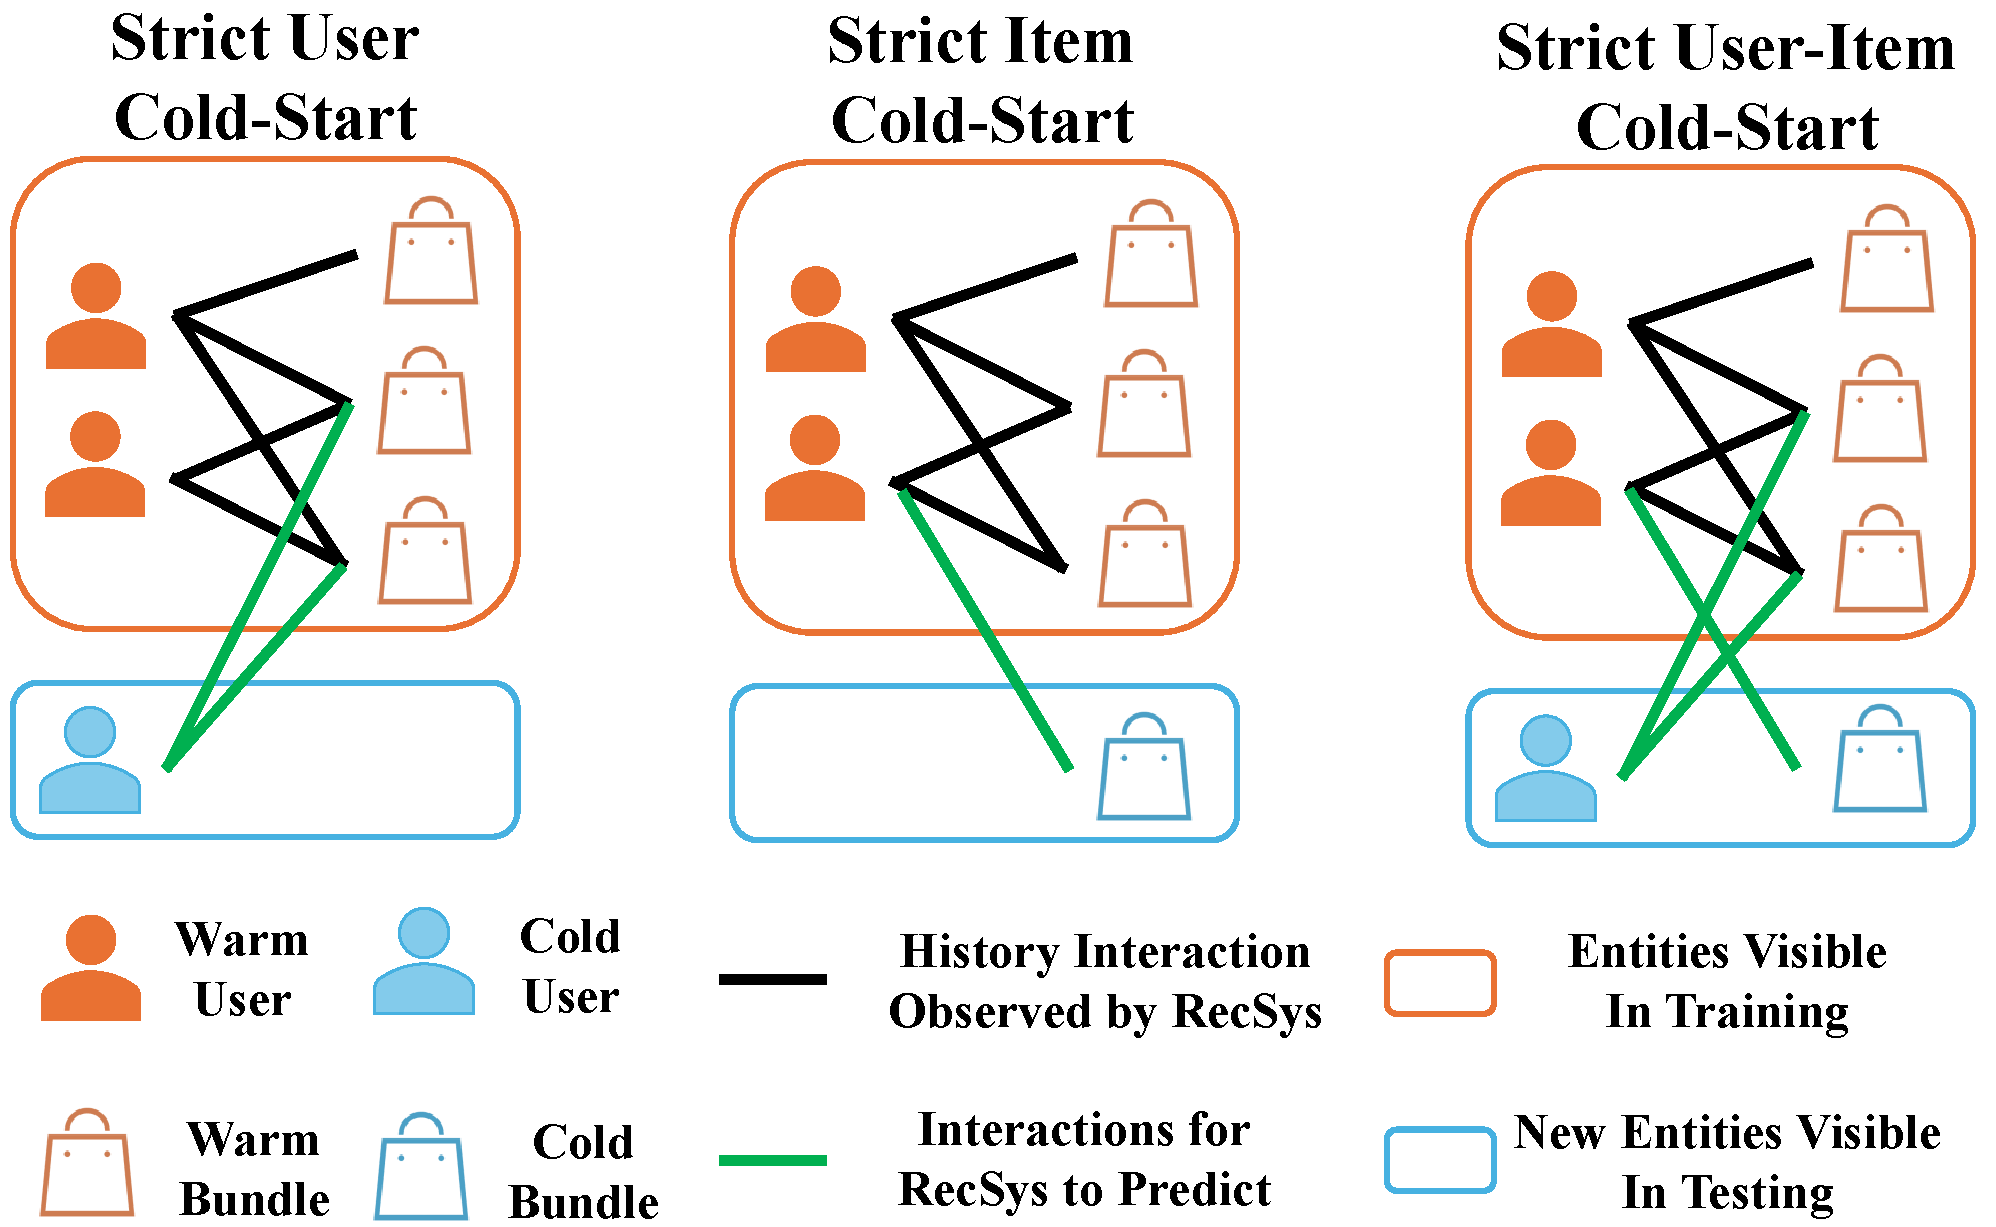
\includegraphics[width=0.4\textwidth]{figures/cold_start.pdf}
  \caption{Comparison of different cold-start recommendation scenarios. We focus on the \textbf{Strict Bundle Cold-Start} setting (middle), where new bundles have no historical interactions (black lines) during training, making it difficult for graph models to predict future interactions (green lines).}
  \label{fig:cold_start}
\end{figure}



However, existing methods exhibit limited robustness in handling cold-start bundle recommendation, particularly the \textbf{strict bundle cold-start} recommendation~\cite{sun2024survey}, since they rely on sufficient information among users, items, and bundles. In real-world scenarios, the interaction space is highly sparse and follows a long-tail distribution. Traditional discriminative models, depending heavily on sufficient historical interactions (warm-start settings), struggle to learn effective representations for newly created bundles that have insufficient interactions. As illustrated in Figure~\ref{fig:cold_start}, the reliance on historical interactions makes graph-based methods ineffective for disconnected nodes. Furthermore, user preferences for bundles are often driven by complex, entangled intents, such as purchasing for utility versus aesthetics, as shown in Figure~\ref{fig:bundle_rec}. Existing graph-based methods often fail to disentangle these fine-grained interests, leading to suboptimal performance when generalizing to unseen bundles.



To tackle these issues, we propose a novel generative framework named \textbf{DDBR} (personalized \textbf{D}iscrete \textbf{D}iffusion Model for cold-start \textbf{B}undle \textbf{R}ecommendation). Inspired by the outstanding performance of diffusion models in generative tasks~\cite{bui2025personalized}, we propose a paradigm shift from discriminating existing interactions to generating robust preferences for recommending \revise{strict cold-start bundles} for users. \revise{Unlike prior generative approaches such as DisCo~\cite{bui2025personalized} that operate in a continuous latent space and generate real-valued item distributions (which are distributionally mismatched with the binary bundle-item affiliation), DDBR employs a discrete Bernoulli diffusion process that natively models the binary nature of bundle-item compositions. This design avoids the continuous-to-discrete mismatch and enables more precise modeling of item presence/absence patterns.} Specifically, we design a personalized discrete diffusion backbone tailored for bundle recommendation to generate a discrete bundle representation. It is capable of synthesizing potential interactions for cold-start bundles by learning the underlying data distribution. To address the complexity of user decision-making, we incorporate a Mamba-based disentangled interest mechanism to guide the diffusion process. Owing to its input-dependent selection mechanism, the Mamba architecture acts as an adaptive noise filter that sharpens the distinctiveness of fine-grained user interests while suppressing GCN-induced aggregation noise. This allows the model to capture specific facets of user intent, effectively distinguishing between diverse motivations behind interactions. By synthesizing robust representations in the discrete latent space, DDBR effectively bridges the connectivity gap caused by extreme data sparsity. Extensive experiments across 3 real-world datasets, including Youshu, iFashion, and Meal, demonstrate that DDBR outperforms multiple advanced baselines, showing the superiority of DDBR in recommending \revise{strict cold-start bundles}.


\begin{figure}[t]
\centering
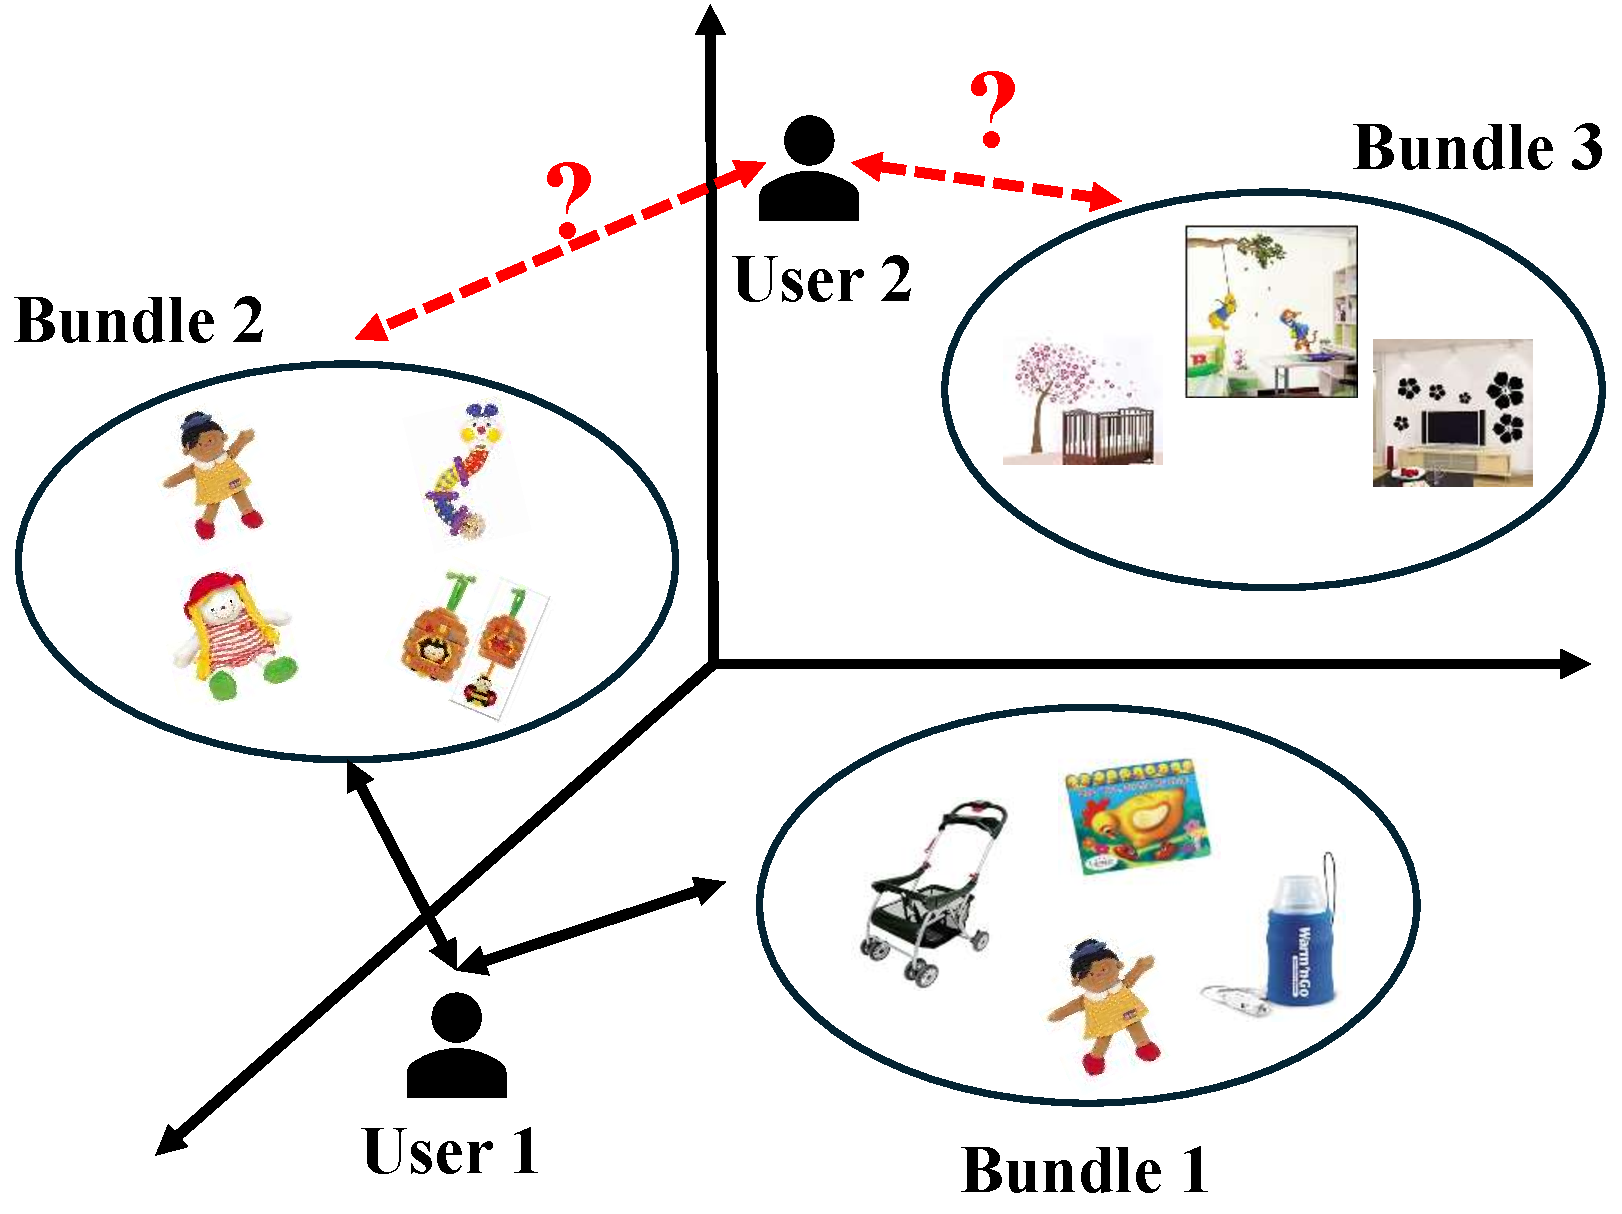
\includegraphics[width=0.4\textwidth]{figures/bundle_rec.pdf}
  \caption{An illustration of the bundle recommendation challenge. User 1 has purchased Bundle 1 (baby necessities) and Bundle 2 (toys). User 2 has purchased Bundle 1. To accurately recommend the next bundle (functional toys in Bundle 2 vs. room decoration in Bundle 3) to User 2, the system must disentangle the specific user interests driving the purchase.}
  \label{fig:bundle_rec}
\end{figure}

To summarize, the key contributions are outlined as follows.
\begin{itemize}
\item \revise{We propose \textbf{DDBR}, a ``Generate-then-Match'' framework for strict bundle cold-start recommendation, whose core is a Conditional Discrete Diffusion Generator (CDDG) that synthesizes an ideal bundle vector natively in the binary item space, removing the dependence on historical user-bundle connectivity.}
\item \revise{We design a Graph-based Representation Learning (GRL) module with dual-level (inter- and intra-view) disentangled contrastive learning, and a Mamba-based Disentangled Preference Encoder (DPE) whose selective-scan mechanism acts as an adaptive noise filter to decouple fine-grained user intents; architecture ablations (MLP/GRU/Self-Attention) validate this choice.}
\item \revise{We establish a rigorous strict bundle cold-start evaluation protocol and validate DDBR on 3 real-world benchmarks through extensive comparisons, ablation studies, hyperparameter analyses, and qualitative visualizations that collectively substantiate each design choice.}
\end{itemize}


\section{Related Work}

%\subsection{Bundle Recommendation}
\noindent\textbf{Bundle Recommendation.}
Bundle recommendation is pivotal for enhancing user experience and platform revenue~\cite{sun2024survey}. Existing approaches predominantly fall into the \textit{discriminative paradigm}, evolving from early factorization models~\cite{cao2017embedding, pathak2017generating} to Graph Neural Networks (GNNs)~\cite{chang2020bundle, wei2023strategy,lei2025feature,kim2024content} and recent contrastive learning frameworks~\cite{ma2022crosscbr, ma2024multicbr}. While these methods effectively capture user preferences by maximizing view consistency on dense graphs, they rely heavily on historical interactions, suffering severely in \textit{cold-start} scenarios where new bundles lack connectivity records~\cite{jeon2024cold}. To mitigate this, a nascent \textit{generative paradigm} has emerged. DisCo~\cite{bui2025personalized} makes the first attempt to use continuous diffusion models with disentangled user interests for cold-start bundle recommendation, demonstrating the promise of generative approaches. \revise{However, DisCo operates in a continuous latent space and generates real-valued item distributions, which are distributionally mismatched with the binary nature of bundle-item compositions and must be matched to binary composition vectors over misaligned spaces.} In contrast, our DDBR leverages the generative capability of discrete Bernoulli diffusion models to infer latent interaction distributions for cold bundles directly in the native binary space, bridging the gap between content and collaborative signals \revise{without this continuous-to-discrete mismatch}.

\noindent\textbf{Cold-Start Recommendation.}
Cold-Start Recommendation (CSR) remains a longstanding challenge. A comprehensive survey~\cite{zhang2025cold} categorizes CSR methods by their external knowledge usage. Early works focused on \textit{data-incomplete learning}, which often employs meta-learning~\cite{lee2019melu,wang2023preference,pang2022pnmta} or Domain Knowledge Transfer techniques~\cite{wang2025integrating,vajjala2024vietoris,zhu2022personalized} to simulate cold scenarios. With the rise of GNNs, researchers shifted to exploiting higher-order graph relations~\cite{hu2020heterogeneous} and cross-domain transfer~\cite{zhu2021transfer} to refine cold node embeddings. Recently, Large Language Models (LLMs) have triggered a paradigm shift by utilizing world knowledge for zero-shot recommendations~\cite{bao2023tallrec, wei2024generative,li2025llm,liang2025taxonomy}. Despite their promise, LLMs suffer from high inference latency and computational costs. Besides, for cold-start bundle recommendation, specialized approaches remain scarce. CoHeat~\cite{jeon2024cold} employs hyperbolic contrastive learning to address sparsity, while CLCRec~\cite{wei2021contrastive} leverages contrastive signals across user-item and user-bundle views. \revise{CVAE-based methods~\cite{zhao2022cvae,bai2023gorec} generate warm-up representations for cold items} through conditional variational inference, but their continuous latent space modeling limits their ability to capture the discrete nature of bundle compositions. This motivates the exploration of \textit{efficient generative alternatives}. Unlike previous works relying on heavy LLMs or external auxiliary data, we propose a discrete diffusion-based approach that endogenously generates robust representations for cold-start bundles by learning the underlying data distribution.


\noindent\textbf{Diffusion Models for Recommendation.}
Diffusion Models (DMs) have achieved remarkable success in generative tasks~\cite{ho2020denoising,yang2023diffusion} and are increasingly applied to recommender systems~\cite{ho2020denoising,huang2024dual,jiang2024diffairec,zang2025diffusion}. Pioneering works~\cite{li2023diffurec,bui2025personalized,walker2022recommendation,zhu2025ld4mrec}  treat interaction prediction as a corrupted-image generation process, significantly outperforming traditional GANs and VAEs. Subsequent studies have extended DMs to sequence recommendation~\cite{li2023diffurec,xie2024bridging,qin2023diffusion} and knowledge graph enhancement~\cite{jiang2024diffkg}. However, most existing diffusion-based recommenders operate on continuous latent spaces or user-item bipartite graphs, failing to address the specific challenges of \textit{bundle recommendation}, such as the discrete nature of bundle-item affiliations and the hierarchical structure of user-bundle interactions. To the best of our knowledge, DDBR is the first to tailor a discrete diffusion framework specifically for the strict bundle cold-start problem.

\revise{\noindent\textbf{Why DDBR vs.\ Existing Cold-Start Methods.} Relative to prior cold-start recommenders, DDBR offers three distinguishing advantages: (i) it requires no U-B message passing at inference, so it naturally serves bundles with zero interactions, unlike GNN-based methods (CrossCBR, MultiCBR, CoHeat); (ii) it requires no external item features or LLM world knowledge, unlike feature-based (CVAR, CLCRec) and LLM-based (TALLRec) methods, keeping inference self-contained and lightweight; and (iii) it models bundle composition natively in the discrete Bernoulli space, avoiding the real-valued/binary mismatch of continuous generative methods (DisCo).}
%,qin2023diffusion
\section{Methodology}
\begin{figure*}[t]
\centering
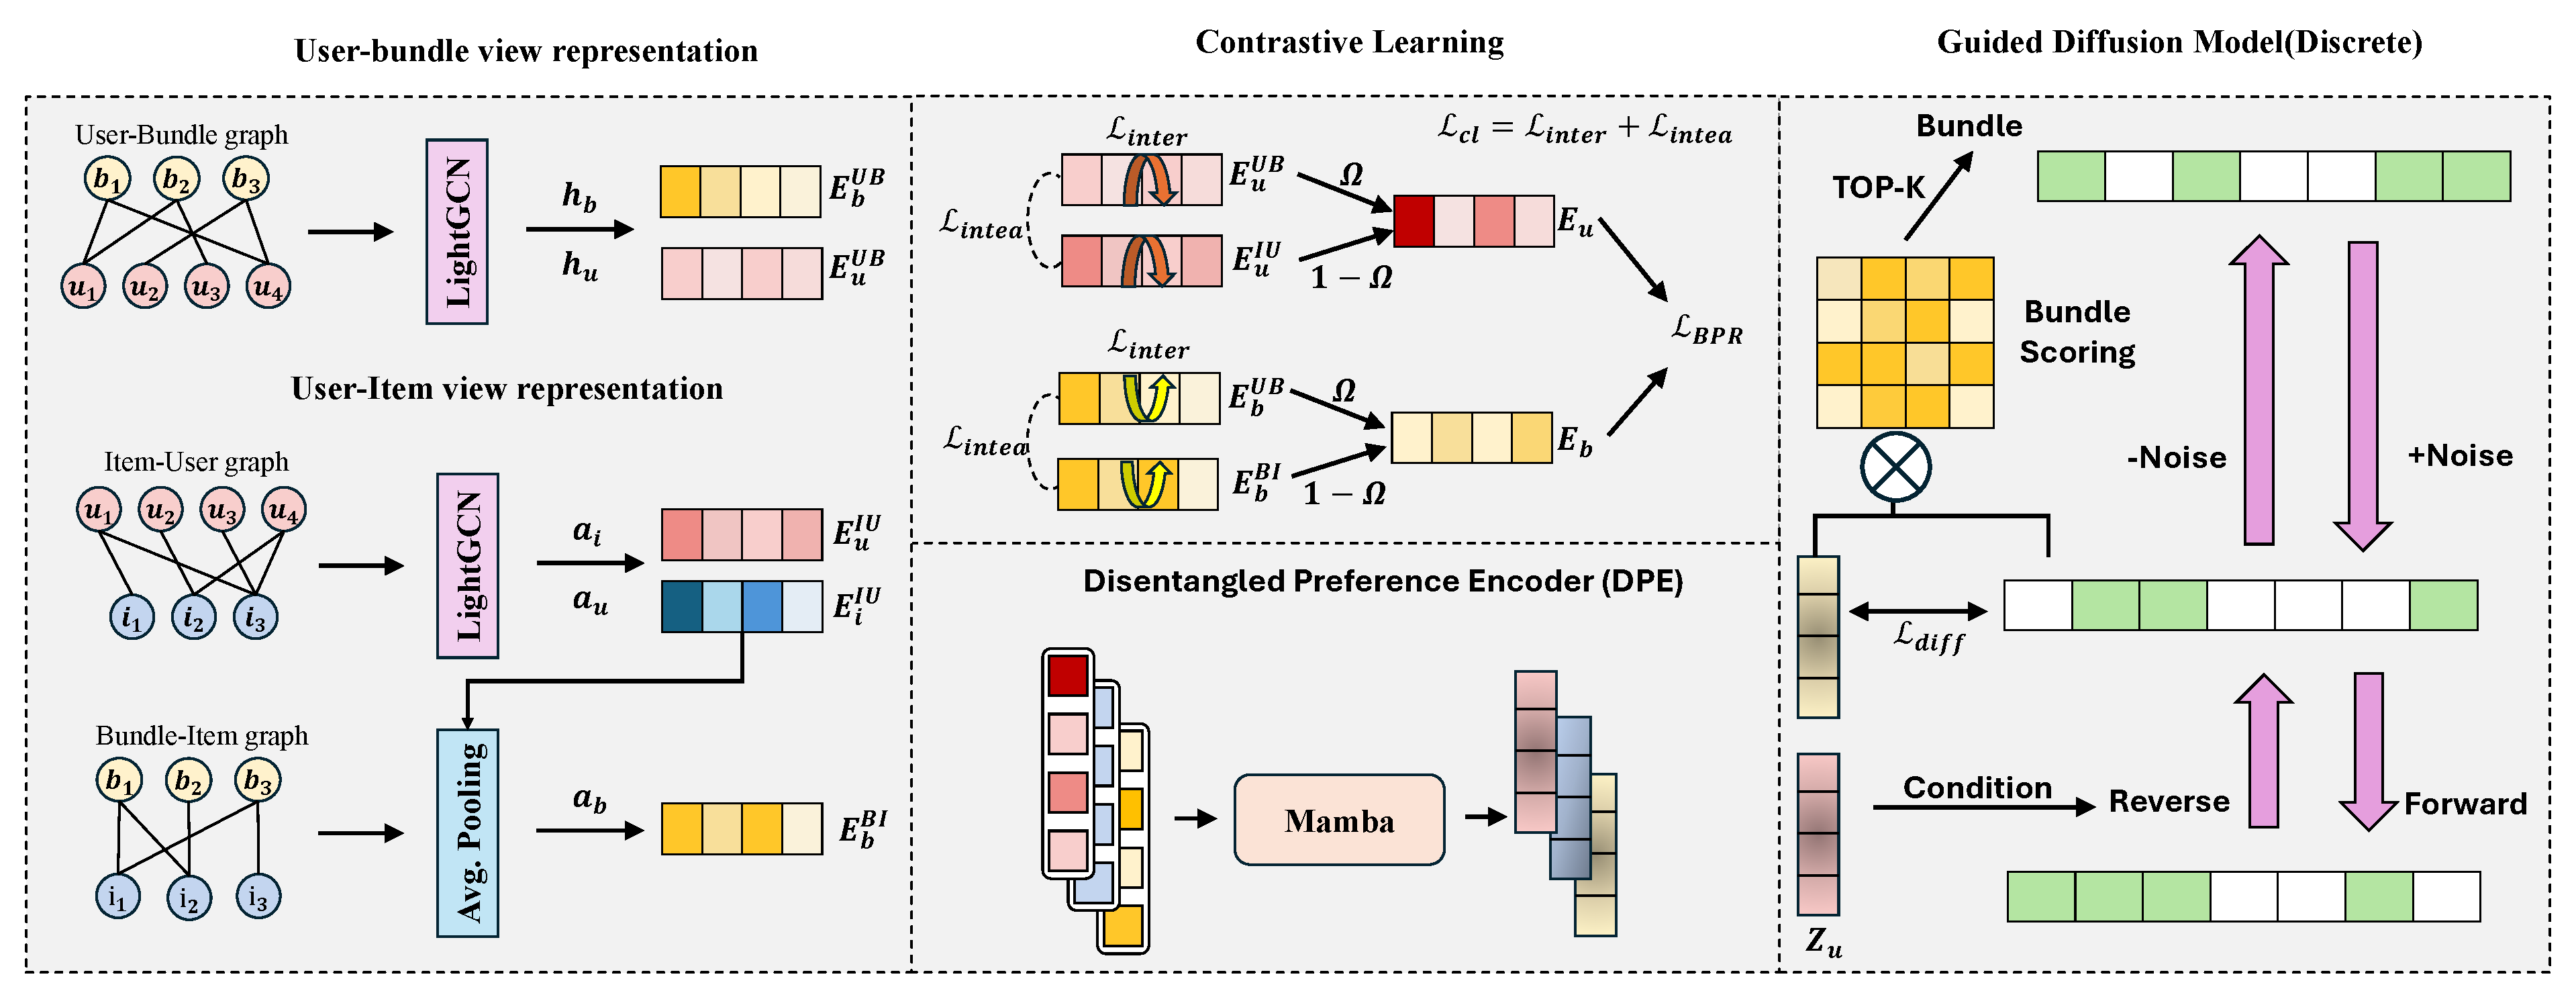
\includegraphics[width=0.99\textwidth]{figures/overviewall.pdf}
  \caption{An overview of our proposed model for DDBR. It learns dual user/bundle embeddings via LightGCN on collaborative and affiliation graphs. A Mamba-based Disentangled Preference Encoder (DPE) refines these inputs into a unified preference vector. This representation then guides a discrete Diffusion Model to generatively produce a high-quality personalized bundle. Finally, we compute the similarity score between the generated bundle and existing bundles to return the top-$k$ recommended bundles. }
  \label{fig:overview}
\end{figure*}
In this section, we present the proposed \textbf{DDBR} framework. Unlike traditional discriminative methods that rely on historical connectivity and struggle with unseen bundles, DDBR operates in a novel \textbf{``Generate-then-Match''} paradigm tailored for the strict cold-start setting. 
Specifically, the framework first employs a conditional discrete diffusion mechanism to synthesize an \textit{ideal bundle vector} representing the user's latent intent, and subsequently retrieves the most similar candidate cold bundles via efficient dot-product matching.
As illustrated in Figure~\ref{fig:overview}, the architecture consists of three synergized components: a collaborative graph encoder, a Mamba-based disentangled preference model, and a discrete diffusion generator, followed by a composite training objective designed to optimize both generative fidelity and ranking accuracy.

\subsection{Problem Formulation}
Let $\mathcal{U}$, $\mathcal{I}$, and $\mathcal{B}$ denote the sets of users, items, and bundles, respectively. We model the relations among these entities using three bipartite graphs that are defined by their sparse adjacency matrices. The first is \textbf{User-Item Graph $\mathbf{A}_{ui} \in \{0,1\}^{|\mathcal{U}| \times |\mathcal{I}|}$}, where $\mathbf{A}_{ui}(u,i)=1$ indicates that user $u$ has historically interacted with item $i$. Let $\mathbf{x}_u \in \{0,1\}^{|\mathcal{I}|}$ denote the $u$-th row of $\mathbf{A}_{ui}$, it represents user $u$'s prior item preferences. The second is \textbf{User-Bundle Graph $\mathbf{A}_{ub} \in \{0,1\}^{|\mathcal{U}| \times |\mathcal{B}|}$}. It represents the observed user-bundle interactions. The third is \textbf{Bundle-Item Graph $\mathbf{A}_{bi} \in \{0,1\}^{|\mathcal{B}| \times |\mathcal{I}|}$}, where $A_{bi}(b,i)=1$ signifies that item $i$ is a constituent of bundle $b$.

\noindent \textbf{Strict Bundle Cold-Start Scenario.}
\revise{We formally define \emph{strict bundle cold-start} as the setting where each test bundle has \emph{no} user-bundle interaction records during training, while its item composition (the bundle-item affiliation matrix $\mathbf{A}_{bi}$) remains known as static metadata---this is a \emph{composition-aware} cold-start setting, stricter than content-based cold-start yet more practical than a fully information-free scenario.} In this work, we focus on addressing the strict bundle cold-start setting, where the bundle set is partitioned into disjoint training and testing sets, that is, $\mathcal{B} = \mathcal{B}_{\text{train}} \cup \mathcal{B}_{\text{test}}$ and $\mathcal{B}_{\text{train}} \cap \mathcal{B}_{\text{test}} = \emptyset$.
During the training phase, the following information is accessible: (i) the full user-item interaction history $\mathbf{A}_{ui}$, which captures all historical item-level preferences; (ii) the bundle-item affiliation matrix $\mathbf{A}_{bi}$, which describes the static composition structure of each bundle and serves as inherent metadata rather than collaborative interaction data, analogous to item attributes in content-based cold-start scenarios; and (iii) the user-bundle interactions $\mathbf{A}_{ub}^{\text{train}}$ restricted exclusively to training bundles $\mathcal{B}_{\text{train}}$. Bundles in $\mathcal{B}_{\text{test}}$ have zero user-bundle interaction records during training and are completely absent from the user-bundle interaction matrix $\mathbf{A}_{ub}^{\text{train}}$. Notably, our formulation is even stricter than most existing cold-start literature, as we assume zero cross-bundle collaborative signals for test bundles.

\noindent \textbf{Task Definition.}
Given a user $u$ and their historical item preference $\mathbf{x}_u$, the goal is to learn a generative mapping that predicts an optimal bundle composition vector $\hat{\mathbf{y}}_u \in \mathbb{R}^{|\mathcal{I}|}$.
During inference, this generated vector $\hat{\mathbf{y}}_u$ is matched against the ground-truth compositions of candidate bundles in $\mathcal{B}_{\text{test}}$ (via $\mathbf{A}_{bi}$) to produce a ranked list of recommendations. Critically, since $\mathbf{A}_{bi}$ encodes static bundle composition metadata rather than user interaction signals, it is fully observed for both training and test bundles, enabling the model to compute bundle representations on-the-fly via mean-pooling of constituent item embeddings during inference. \revise{Importantly, although $\mathbf{A}_{bi}$ is fully observed, only the B-I rows of \emph{training} bundles are used during training (for graph construction and as diffusion targets); the compositions of test bundles are used exclusively at inference for scoring, so test bundles remain truly unseen during training.}

\subsection{Model Design}
To achieve this objective, DDBR integrates three core modules: 
i) A \textbf{Graph-based Representation Learning (GRL)} module that synergizes a Collaborative Graph Encoder with Dual-Level Disentangled Contrastive Learning. This module extracts high-order collaborative signals while refining user representations through inter-view and intra-view consistency constraints, effectively mitigating noise and sparsity to yield robust, high-quality embeddings. 
ii) A \textbf{Mamba-based Disentangled Preference Encoder (DPE)} that efficiently captures multi-faceted user interests with linear complexity, serving as the conditional guiding signal. iii) A \textbf{Conditional Discrete Diffusion Generator (CDDG)} that operates directly on the discrete Bernoulli space to synthesize the user's ideal bundle vector $\hat{\mathbf{x}}_{\text{ideal}}$, avoiding the \revise{real-valued/binary mismatch} of continuous diffusion models.

%\subsection{Graph Contrastive Representation Learning}
\subsubsection{Graph-based Representation Learning}
\noindent \textbf{Graph-based Representation.}
Our framework extracts comprehensive collaborative representations for users, items, and bundles from three distinct views: the User-Bundle (UB) view, the User-Item (UI) view, and the Bundle-Item (BI) view. We employ LightGCN~\cite{he2020lightgcn} to extract latent features from the user-bundle graph $\mathcal{G}_{ub}$ and user-item graph $\mathcal{G}_{ui}$. Let $\mathbf{E}^{(0)}$ denote the initial ID embeddings. The graph propagation at layer $l$ aggregates neighbor information as follows:
\begin{equation}
    \mathbf{e}_{u}^{(l+1)} = \sum_{v \in \mathcal{N}_u} \frac{1}{\sqrt{|\mathcal{N}_u||\mathcal{N}_v|}} \mathbf{e}_{v}^{(l)},
\end{equation}
where $v$ represents the connected node like bundle $b$ in $\mathcal{G}_{ub}$ or item $i$ in $\mathcal{G}_{ui}$. After $L$  layers, we obtain the final representations via mean pooling. Consequently, we derive the user and bundle representations $\mathbf{E}_u^{UB}$ and $\mathbf{E}_b^{UB}$ from $\mathcal{G}_{ub}$. Similarly, we obtain the user representations $\mathbf{E}_u^{IU}$ and item representations $\mathbf{E}_i^{IU}$ from $\mathcal{G}_{ui}$.

\revise{We clarify that the LightGCN message passing over $\mathcal{G}_{ub}$ is performed \emph{only during training}, to learn user and bundle embeddings and to supervise the BPR and contrastive objectives. At inference, no U-B propagation is performed: the learned user embedding is fixed, and a cold bundle is scored using only its B-I composition (Sec.~\ref{sec:inference}). Thus, recommending a test bundle never requires any U-B interaction of that bundle.}

To explicitly model the affiliation between bundles and items, we construct the bundle-item graph $\mathcal{G}_{bi}$ \revise{using only the B-I affiliations of training bundles}. Since a bundle is semantically defined by its constituent items, we aggregate the embeddings of items belonging to bundle $b$ to form the bundle's view representation as follows:
\begin{equation}
    \mathbf{E}_b^{BI} = \frac{1}{|\mathcal{N}_b|} \sum_{i \in \mathcal{N}_b} \mathbf{E}_i^{IU},
\end{equation}
where $\mathcal{N}_b$ is the set of items in bundle $b$. This effectively transfers item-level collaborative signals into the bundle domain.

%\subsection{Collaborative Graph Encoding}
%Our framework constructs representations from three distinct views to capture comprehensive collaborative signals: the User-Bundle (UB) view, the User-Item (UI) view, and the Bundle-Item (BI) view.

%\subsubsection{Triple-View Representation}
%We employ LightGCN~\cite{he2020lightgcn} as the backbone encoder to extract latent features from the user-bundle graph $\mathcal{G}_{ub}$ and user-item graph $\mathcal{G}_{ui}$. 
%Let $\mathbf{E}^{(0)}$ denote the initial ID embeddings. The graph propagation at layer $l$ aggregates neighbor information as follows:
%\begin{equation}
%    \mathbf{e}_{u}^{(l+1)} = \sum_{v \in \mathcal{N}_u} \frac{1}{\sqrt{|\mathcal{N}_u||\mathcal{N}_v|}} \mathbf{e}_{v}^{(l)},
%\end{equation}
%where $v$ represents the connected node (i.e., bundle $b$ in $\mathcal{G}_{ub}$ or item $i$ in $\mathcal{G}_{ui}$). After $L$ layers, we obtain the final representations via mean pooling.
%Consequently, we derive the user and bundle representations from $\mathcal{G}_{ub}$ denoted as $\mathbf{E}_u^{UB}$ and $\mathbf{E}_b^{UB}$, respectively. Similarly, from $\mathcal{G}_{ui}$, we obtain the user representation $\mathbf{E}_u^{IU}$ and item representations $\mathbf{E}_i^{IU}$.

%To explicitly model the affiliation between bundles and items, we construct the bundle-item graph $\mathcal{G}_{bi}$. Since a bundle is semantically defined by its constituent items, we aggregate the embeddings of items belonging to bundle $b$ to form the bundle's view representation:
%\begin{equation}
%    \mathbf{E}_b^{BI} = \frac{1}{|\mathcal{N}_b|} \sum_{i \in \mathcal{N}_b} \mathbf{E}_i^{IU},
%\end{equation}
%where $\mathcal{N}_b$ is the set of items in bundle $b$. This effectively transfers item-level collaborative signals into the bundle domain.

\noindent \textbf{Dual-Level Disentangled Contrastive Learning.}
To mitigate data sparsity and noise, we introduce a dual-level disentangled contrastive learning to refine user representations and bundle representations by maximizing consistency at both the \textit{inter-view} and \textit{intra-view} levels. We employ the InfoNCE loss to align these representations. At the \textbf{inter-view level}, we maximize the mutual information between the shared user semantics from the UB and UI views and the mutual information between the shared bundle semantics from UB and BI views. At the \textbf{intra-view level}, we enforce structural consistency within each view to ensure robustness against local perturbations.

%\subsection{Dual-Level Disentangled Contrastive Learning}
%To mitigate data sparsity and noise, we introduce a dual-level disentangled contrastive learning paradigm. This module refines representations by maximizing consistency at both the \textit{inter-view} and \textit{intra-view} levels.

%\subsubsection{Inter-view and Intra-view Objectives}
%We employ the InfoNCE loss to align representations. 
%At the \textbf{inter-view level}, we maximize the mutual information between the shared user semantics from the UB and UI views (and similarly for bundles between UB and BI views). 
%At the \textbf{intra-view level}, we enforce structural consistency within each view to ensure robustness against local perturbations. 
Formally, the contrastive loss $\mathcal{L}_{cl}$ is defined to minimize the distance between positive pairs while pushing apart negative pairs across these views:
%\begin{equation}
%\mathcal{L}_{cl} = \sum_{v \in \mathcal{V}} -\log \frac{\exp(\text{sim}(\mathbf{e}_v, \mathbf{e}_v^+)/\tau)}{\revise{\exp(\text{sim}(\mathbf{e}_v, \mathbf{e}_v^+)/\tau) + \sum_{k \in \mathcal{N}_v} \exp(\text{sim}(\mathbf{e}_v, \mathbf{e}_k^-)/\tau)}},
%\label{eq:cl}
%\end{equation}
\begin{equation}
\begin{aligned}
& \mathcal{L}_{cl}= \sum_{v \in \mathcal{V}} -\log d_{\mathbf{e}_v}, \\
& d_{\mathbf{e}_v}= \frac{\exp(\text{sim}(\mathbf{e}_v, \mathbf{e}_v^+)/\tau)}{\exp(\text{sim}(\mathbf{e}_v, \mathbf{e}_v^+)/\tau) + \sum_{k \in \mathcal{N}_v} \exp(\text{sim}(\mathbf{e}_v, \mathbf{e}_k^-)/\tau)},
\end{aligned}
\label{eq:cl}
\end{equation}
where $\mathcal{V}$ encompasses the node sets for both inter-view and intra-view comparisons, $\mathcal{N}_v$ is the set of negative samples, and $\tau$ is the temperature parameter controlling discrimination sensitivity.

%\subsubsection{Adaptive View Fusion}
\noindent \textbf{Adaptive View Fusion.}
For the final recommendation task, we adaptively fuse the refined representations from different views. A learnable parameter $\Omega \in [0,1]$ is introduced to balance the contribution of each view based on its reliability:
\begin{equation}
\begin{aligned}
    \mathbf{E}_u &= \Omega \mathbf{E}_u^{UB} + (1 - \Omega) \mathbf{E}_u^{IU}, \\
    \mathbf{E}_b &= \Omega \mathbf{E}_b^{UB} + (1 - \Omega) \mathbf{E}_b^{BI}.
\end{aligned}
\end{equation}
These fused embeddings $\mathbf{E}_u$ and $\mathbf{E}_b$ encompass multi-view collaborative signals and serve as the input for the BPR optimization and the subsequent conditional diffusion process.

\subsubsection{Disentangled Preference Encoder}
\label{sec:disentangled_mamba}
While the GRL captures high-order collaborative signals, the resulting user embeddings still suffer from the \textit{entanglement} of latent intents, like the intertwined sensitivity to price, category, and style. Standard attention mechanisms can model dependencies but lack explicit noise filtering capabilities. To address this, we introduce a \textbf{Mamba-based Disentangled Preference Encoder}. Our choice of Mamba over simpler alternatives is motivated by two key considerations: (i) the input-dependent selection mechanism of the Selective State Space Model (SSM)~\cite{gu2024mamba} can naturally act as an adaptive noise filter, allowing the model to dynamically emphasize salient interest factors while suppressing GCN-induced aggregation noise, which is a capability that static MLPs and fixed-transition RNNs lack; and (ii) the state-space formulation provides a structured inductive bias for modeling the sequential dependencies among latent preference factors, outperforming standard self-attention when the number of factors $K$ is small. \revise{We emphasize that DDBR exploits Mamba for its \emph{input-dependent selection} (gating) rather than its linear-complexity scaling over long sequences: the sequence being modeled is the short sequence of $K$ latent preference factors---not the user's (sparse) interaction history---so the relevant property is adaptive noise filtering, not asymptotic efficiency.} We provide empirical validation of this design choice through architecture ablation experiments in Section~\ref{sec:ablation}.

%We leverage the Selective State Space Model (SSM)~\cite{gu2024mamba} not merely for its linear efficiency, but primarily for its \textit{input-dependent selection mechanism}, which allows the model to adaptively highlight salient interest factors while suppressing irrelevant interaction noise.

%\subsubsection{Latent Interest Factorization}
\noindent \textbf{Latent User Preference Factorization.}
We postulate that a user's global representation $\mathbf{E}_u$ is a composite of $K$ distinct latent preference factors. To model these factors, we project the unified embedding into a latent factor sequence by partitioning the embedding space as follows:
\begin{equation}
\label{eq:mamba_disentangle}
\begin{split}
    \mathbf{E}_u \in \mathbb{R}^{d} \;&\xrightarrow{\text{View}}\; \mathbf{S}_u \\
    &= [\mathbf{s}_u^{(1)}, \dots, \mathbf{s}_u^{(K)}] \in \mathbb{R}^{K \times d_k},
\end{split}
\end{equation}
where $d = K \times d_k$ and $\mathbf{s}_u^{(k)}$ represents a specific subspace of user preference. 
%, initialized but yet to be refined by contextual dependencies.

%\subsubsection{Selective Aspect Modeling}
\noindent \textbf{Selective Aspect Modeling.}
We employ a Mamba block to model the dynamic correlations among these latent factors. The core innovation lies in the \textit{Selective Scan}, which governs how information propagates across the preference sequence.
Unlike static transition matrices in RNNs, Mamba derives continuous parameters $(\mathbf{\Delta}, \mathbf{B}, \mathbf{C})$ directly from the input interest token $\mathbf{s}_u^{(k)}$:
\begin{equation}
\label{eq:mamba_core}
\begin{split}
    \mathbf{h}_k &= \bar{\mathbf{A}} \mathbf{h}_{k-1} + \bar{\mathbf{B}}_k \mathbf{s}_u^{(k)}, \\
    \mathbf{y}_k &= \mathbf{C}_k \mathbf{h}_k,
\end{split}
\end{equation}
where $\bar{\mathbf{A}}$ and $\bar{\mathbf{B}}_k$ are the discretized state transition parameters derived via $\mathbf{\Delta}_k$.
In the context of recommendation, $\mathbf{\Delta}_k$ acts as a gating mechanism to determine how much focus to retain on the current preference factor $\mathbf{s}_u^{(k)}$ versus the accumulated historical context $\mathbf{h}_{k-1}$. This enables the encoder to effectively filter out noise introduced by the GCN aggregation and sharpen the distinctiveness of each latent interest.
The refined features are obtained via a residual connection and a Feed-Forward Network (FFN): $\mathbf{Z}_u = \text{FFN}(\text{LayerNorm}(\mathbf{S}_u + \text{Mamba}(\mathbf{S}_u)))$.
%\begin{equation}
%\mathbf{Z}_u = \text{FFN}(\text{LayerNorm}(\mathbf{S}_u + \text{Mamba}(\mathbf{S}_u))),
%\end{equation}

%\subsubsection{Condition Recomposition}
After refining the latent factors, we fuse the disentangled aspects back into a unified condition vector $\mathbf{z}_u = \operatorname{Flatten}(\mathbf{Z}_u) \in \mathbb{R}^{d}$. This recomposition ensures that the final representation encapsulates a structured understanding of user preferences.
%\begin{equation}
%\label{eq:mamba_recompose}
%\mathbf{z}_u = \operatorname{Flatten}(\mathbf{Z}_u) \in \mathbb{R}^{d}.
%\end{equation}
The resulting $\mathbf{z}_u$ serves as a noise-resilient and semantically rich condition to guide the subsequent diffusion generator to synthesize optimal bundles.
\subsection{Guided Discrete Diffusion Model}
\label{sec:diffusion}

Building upon the disentangled user preference representation $\mathbf{z}_u$ derived from the DPE, we propose a Conditional Discrete Diffusion Generator (CDDG). Unlike continuous diffusion models that map discrete data into a real-valued Gaussian space, which often leads to quantization errors and blurring artifacts, our module operates directly within the native discrete binary space $\{0, 1\}^{|\mathcal{I}|}$. This allows DDBR to accurately model the "bit-flipping" nature of items in bundles.
We conceptualize the bundle generation as a reverse denoising process, where the model iteratively refines a noisy Bernoulli distribution into a deterministic bundle structure $\mathbf{x}_0 \in \{0, 1\}^{|\mathcal{I}|}$, conditioned on the user's latent intent $\mathbf{z}_u$.

\noindent\textbf{Ground-Truth Construction.}
For a user who has interacted with multiple historical bundles, we randomly sample a single bundle from their interaction history to serve as the training target $\mathbf{x}_0$. Specifically, each training instance is constructed by drawing one user-bundle interaction pair $(u, b)$ from $\mathbf{A}_{ub}^{\text{train}}$, and the ground-truth vector $\mathbf{x}_0 \in \{0,1\}^{|\mathcal{I}|}$ is defined as the $b$-th row of $\mathbf{A}_{bi}$, i.e., $x_0^{(i)} = 1$ if item $i$ belongs to bundle $b$ and $0$ otherwise. Crucially, we do not perform any union or aggregation over multiple historical bundles. Each $\mathbf{x}_0$ corresponds to exactly one bundle. This design aligns with the generative nature of our framework, enabling the model to learn the distribution of plausible bundle compositions conditioned on user preferences.

\noindent\textbf{Denoising Network Architecture.}
The denoising network $f_\theta$ comprises three components: (i) \textbf{Noise Encoding:} The noisy binary vector $\mathbf{x}_t \in \{0,1\}^{|\mathcal{I}|}$ is first projected through a dedicated embedding layer $\text{Emb}_{\text{noise}}: \{0,1\}^{|\mathcal{I}|} \to \mathbb{R}^{|\mathcal{I}| \times d_{\text{model}}}$ that maps each binary item indicator into a $d_{\text{model}}$-dimensional latent representation, preserving the discrete semantics of bundle composition. (ii) \textbf{Timestep Conditioning:} The diffusion timestep $t$ is encoded via standard sinusoidal positional embeddings followed by a two-layer MLP, producing $\mathbf{e}_t \in \mathbb{R}^{d_{\text{model}}}$. This timestep embedding is integrated through adaptive layer normalization (AdaLN) applied to the intermediate features of the denoising backbone, i.e., $\text{AdaLN}(\mathbf{h}, \mathbf{e}_t) = \gamma(\mathbf{e}_t) \odot \mathbf{h} + \beta(\mathbf{e}_t)$, where $\gamma(\cdot)$ and $\beta(\cdot)$ are learnable affine projections, enabling the network to dynamically adjust its denoising behavior according to the noise level. (iii) \textbf{User Conditioning via Cross-Attention:} The user preference representation $\mathbf{z}_u$ serves as the context for a multi-head cross-attention module. At each denoising block, the timestep-conditioned item features attend to $\mathbf{z}_u$ via cross-attention:
\begin{equation}
    \text{CrossAttn}(\mathbf{Q}, \mathbf{K}, \mathbf{V}) = \text{softmax}(\frac{\mathbf{Q}\mathbf{K}^\top}{\sqrt{d_k}})\mathbf{V},
\end{equation}
where $\mathbf{Q}$ is projected from the item features and $\mathbf{K}, \mathbf{V}$ from $\mathbf{z}_u$. This mechanism allows the model to dynamically align the generated bundle content with the user's preference profile at every denoising step. Items are modeled jointly through this cross-attention mechanism, capturing complementarity and substitution patterns among co-occurring items rather than predicting each item independently.

\noindent\textbf{Discrete Forward Process.}
The forward diffusion process is a fixed Markov chain that gradually corrupts the ground-truth bundle $\mathbf{x}_0$ into pure noise. Instead of adding Gaussian noise, we employ a state transition mechanism suitable for binary data. For a bundle vector $\mathbf{x}_t$ at step $t$, the transition probability to step $t+1$ is defined using a variance schedule $\beta_t \in (0, 1)$:
\begin{equation}
    q(\mathbf{x}_t | \mathbf{x}_{t-1}) = \mathcal{B}\left(\mathbf{x}_t; (1 - \beta_t)\mathbf{x}_{t-1} + \frac{\beta_t}{2}\right),
\end{equation}
where $\mathcal{B}(\cdot; \theta)$ denotes the Bernoulli distribution with parameter $\theta$. As $t \to T$, the data distribution $q(\mathbf{x}_T)$ converges to a uniform Bernoulli distribution (random noise), effectively erasing the original structural information. This process naturally handles the sparsity of bundle data without requiring auxiliary embeddings.

\noindent\textbf{Generative Reverse Denoising.}
The reverse process aims to reconstruct the optimal bundle $\mathbf{x}_0$ by reversing the corruption steps. Since the exact reverse posterior $q(\mathbf{x}_{t-1} | \mathbf{x}_t)$ is intractable, we approximate it using a parameterized neural network $p_\theta$. Crucially, we condition this process on the disentangled user representation $\mathbf{z}_u$ to ensure the generated bundle aligns with specific user preferences:
\begin{equation}
    p_\theta(\mathbf{x}_{t-1} | \mathbf{x}_t, \mathbf{z}_u) = \prod_{i=1}^{|\mathcal{I}|} p_\theta(x_{t-1}^{(i)} | \mathbf{x}_t, \mathbf{z}_u),
\end{equation}
where the network predicts the probability of each item $i$ being present at step $t-1$.

To effectively capture the dependencies between items and the user condition, the denoising network incorporates the Mamba-enhanced user vector $\mathbf{z}_u$ via a cross-attention mechanism. Specifically, the model predicts the clean structure $\hat{\mathbf{x}}_0$ from the current noisy state $\mathbf{x}_t$ and time step $t$:
\begin{equation}
    \hat{\mathbf{x}}_0 = f_\theta(\mathbf{x}_t, t, \mathbf{z}_u).
\end{equation}
Using the predicted $\hat{\mathbf{x}}_0$, we compute the posterior transition probabilities to sample $\mathbf{x}_{t-1}$, progressively guiding the chaotic binary noise into a coherent set of items that form the recommended bundle. This "Generate-then-Match" paradigm allows DDBR to synthesize high-quality bundles even in strict cold-start scenarios where historical interaction graphs are disconnected.

\subsection{Optimization Objective}
To ensure that DDBR captures robust user preferences while generating high-fidelity bundle compositions, we optimize the DDBR with a joint objective function in an end-to-end manner. The joint objective integrates recommendation ranking loss ($\mathcal{L}_{\mathrm{rec}}$), disentangled contrastive loss ($\mathcal{L}_{\mathrm{cl}}$), and diffusion loss ($\mathcal{L}_{\mathrm{diff}}$):
\begin{equation}
    \mathcal{L}_{\mathrm{total}} = \mathcal{L}_{\mathrm{rec}} + \lambda_1 \mathcal{L}_{\mathrm{cl}} + \lambda_2 \mathcal{L}_{\mathrm{diff}},
    \label{eq:total_loss}
\end{equation}
where $\lambda_1$ and $\lambda_2$ are hyperparameters balancing the contributions of disentangled representation learning and generative reconstruction.

The recommendation ranking loss ($\mathcal{L}_{\mathrm{rec}}$) is Bayesian Personalized Ranking (BPR), which is based on the relative order of interactions. We assume an observed user-bundle pair $(u, b_i)$ should score higher than an unobserved pair $(u, b_j)$, then $\mathcal{L}_{\mathrm{rec}}$ is defined as follows:
\begin{equation}
    \mathcal{L}_{\mathrm{rec}} = \sum_{(u, b_i, b_j) \in \mathcal{D}} - \ln \sigma(\mathbf{E}_u^\top \mathbf{E}_{b_i} - \mathbf{E}_u^\top \mathbf{E}_{b_j}),
\end{equation}
where $\mathcal{D}$ denotes the training triplets and $\sigma(\cdot)$ is the sigmoid function.

\noindent\textbf{\revise{Connection to the Variational Bound.}}
\revise{We now clarify that the diffusion loss corresponds to a principled variational objective rather than an ad hoc reconstruction term. For discrete diffusion, maximizing the conditional likelihood $p_\theta(\mathbf{x}_0 \mid \mathbf{z}_u)$ is intractable, so we optimize its evidence lower bound (ELBO), which decomposes over timesteps as}
\begin{equation}
\begin{aligned}
-\log p_\theta(\mathbf{x}_0 \mid \mathbf{z}_u) \le \mathbb{E}_{q}\Big[ &\, D_{\mathrm{KL}}\big(q(\mathbf{x}_T \mid \mathbf{x}_0)\,\|\,p(\mathbf{x}_T)\big) \\
&+ \sum_{t=2}^{T} D_{\mathrm{KL}}\big(q(\mathbf{x}_{t-1} \mid \mathbf{x}_t, \mathbf{x}_0)\,\|\,p_\theta(\mathbf{x}_{t-1} \mid \mathbf{x}_t, \mathbf{z}_u)\big) \\
&- \log p_\theta(\mathbf{x}_0 \mid \mathbf{x}_1, \mathbf{z}_u) \Big],
\end{aligned}
\end{equation}
\revise{where the denoising-matching terms reduce to per-item binary cross-entropy between the analytic posterior $q(\mathbf{x}_{t-1} \mid \mathbf{x}_t, \mathbf{x}_0)$ and the predicted distribution $p_\theta$. Our $\mathcal{L}_{\mathrm{BCE}}$ instantiates exactly these per-item cross-entropy terms, with the positive/negative/coverage/exposure components acting as a sparsity-aware reweighting of the same variational objective. This establishes that DDBR performs genuine discrete diffusion modeling rather than an ad hoc denoising autoencoder.}

The diffusion loss ($\mathcal{L}_{\mathrm{diff}}$) aims to reconstruct the ground-truth bundle structure $\mathbf{x}_0$ conditioned on the user intent $\mathbf{z}_u$. To address the extreme sparsity of bundle data where valid items are rare, we employ a composite loss comprising a weighted binary cross-entropy loss $\mathcal{L}_{\mathrm{BCE}}$, a coverage loss $\mathcal{L}_{\mathrm{coverage}}$, and an exposure penalty $\mathcal{L}_{\mathrm{exposure}}$:
\begin{equation}
%\color{blue}
    \mathcal{L}_{\mathrm{diff}} = \mathcal{L}_{\mathrm{BCE}} + \alpha \mathcal{L}_{\mathrm{coverage}} + \beta \mathcal{L}_{\mathrm{exposure}}.
\end{equation}

The weighted binary cross-entropy loss $\mathcal{L}_{\mathrm{BCE}}$ operates on three disjoint sets of items:
\begin{equation}
    \begin{aligned}
    \mathcal{L}_{\mathrm{BCE}} = \mathbb{E}_{t, \mathbf{x}_0} \bigg[ &\sum_{i \in \mathcal{I}^+} - \omega_{\text{pos}} \cdot \log \hat{p}_\theta(x_{0}^{(i)}=1 | \mathbf{x}_t, t, \mathbf{z}_u) \\
    + &\sum_{i \in \mathcal{I}^{\text{hist}}} - \omega_{\text{hist}} \cdot \ell\left(x_{\text{hist}}^{(i)},\; \hat{p}_\theta(x_{0}^{(i)} | \mathbf{x}_t, t, \mathbf{z}_u)\right) \\
    + &\sum_{i \in \mathcal{I}^-} - \omega_{\text{neg}} \cdot \log \hat{p}_\theta(x_{0}^{(i)}=0 | \mathbf{x}_t, t, \mathbf{z}_u) \bigg],
    \end{aligned}
\end{equation}
where $\mathcal{I}^+$ denotes items in the target bundle ($x_0^{(i)}=1$), $\mathcal{I}^{\text{hist}}$ denotes items the user has historically interacted with but are absent from the target bundle, and $\mathcal{I}^-$ denotes items the user has never interacted with. The weight parameters are set as $\omega_{\text{pos}} > \omega_{\text{hist}} > \omega_{\text{neg}}$ to prioritize recall of bundle items while maintaining discriminative pressure on negatives. $\ell(\cdot,\cdot)$ denotes the binary cross-entropy between the historical preference and the prediction.

The coverage loss $\mathcal{L}_{\mathrm{coverage}}$ encourages comprehensive item recall within the bundle:
\begin{equation}
    \mathcal{L}_{\mathrm{coverage}} = \mathbb{E}_{t, \mathbf{x}_0} \bigg[ -\frac{1}{|\mathcal{I}^+|} \sum_{i \in \mathcal{I}^+} \log \hat{p}_\theta(x_{0}^{(i)}=1 | \mathbf{x}_t, t, \mathbf{z}_u) \bigg].
\end{equation}

The exposure penalty $\mathcal{L}_{\mathrm{exposure}}$ discourages over-prediction of negative items:
\begin{equation}
    \mathcal{L}_{\mathrm{exposure}} = \mathbb{E}_{t, \mathbf{x}_0} \bigg[ \frac{1}{|\mathcal{I}^-|} \sum_{i \in \mathcal{I}^-} \hat{p}_\theta(x_{0}^{(i)}=1 | \mathbf{x}_t, t, \mathbf{z}_u) \bigg].
\end{equation}

Here, $\hat{p}_\theta$ is the predicted probability of item presence. The complete formulation ensures that the model not only recalls legitimate bundle items with the help of $\mathcal{L}_{\mathrm{BCE}}$ and $\mathcal{L}_{\mathrm{coverage}}$, but also maintains sparse, realistic predictions with the help of the negative component of $\mathcal{L}_{\mathrm{BCE}}$ and $\mathcal{L}_{\mathrm{exposure}}$. $\alpha$ and $\beta$ are hyperparameters balancing the coverage and exposure regularization terms.

\subsection{Inference and Bundle Matching}
\label{sec:inference}
At inference time, DDBR generates recommendations through the following ``Generate-then-Match'' procedure:

\noindent\textbf{Generation.}
For a target user $u$, the model starts from a random Bernoulli noise vector $\mathbf{x}_T \sim \mathcal{B}(0.5)$ and iteratively applies the learned reverse diffusion process for $T$ steps, conditioned on the user's disentangled preference representation $\mathbf{z}_u$. At each step $t$, the denoising network predicts the clean structure $\hat{\mathbf{x}}_0 = f_\theta(\mathbf{x}_t, t, \mathbf{z}_u)$, and $\mathbf{x}_{t-1}$ is sampled from the posterior $p_\theta(\mathbf{x}_{t-1} | \mathbf{x}_t, \mathbf{z}_u)$. The final output after $T$ reverse steps is an item-level probability vector $\hat{\mathbf{y}}_u \in [0,1]^{|\mathcal{I}|}$, representing the user's preferred item composition for a bundle.

\noindent\textbf{Matching.}
To produce a ranked list of bundle recommendations, we score each candidate bundle $b \in \mathcal{B}_{\text{test}}$ by computing the dot product between the generated item preference vector and the bundle's item composition:
\begin{equation}
\text{score}(u, b) = \hat{\mathbf{y}}_u^\top \cdot \mathbf{A}_{bi}[b, :],
\end{equation}
where $\mathbf{A}_{bi}[b, :]$ is the binary composition vector of bundle $b$. Bundles are then ranked in descending order according to this score.

\noindent\textbf{Handling Unseen Bundles.}
A key design of DDBR is that bundle representations are not stored as embedding vectors. Instead, any bundle, including cold-start bundles in $\mathcal{B}_{\text{test}}$, is represented on-the-fly by mean-pooling the embeddings of its constituent items: 
\begin{equation}
\mathbf{E}_b = \frac{1}{|\mathcal{N}_b|} \sum_{i \in \mathcal{N}_b} \mathbf{E}_i,
\end{equation} 
where $\mathbf{E}_i$ is the item embedding learned from the user-item interaction graph. Since $\mathbf{A}_{bi}$ is fully observed at both training and inference time, there is no ``unseen bundle embedding'' problem. The BPR-based recommendation scoring $\mathbf{E}_u^\top \mathbf{E}_b$ and the diffusion-based matching score $\hat{\mathbf{y}}_u^\top \mathbf{A}_{bi}[b,:]$ are combined via late fusion to produce the final ranking.

%we design a hybrid objective function. This function jointly optimizes the discriminative graph encoder and the generative diffusion model in an end-to-end manner.

%\subsubsection{Discriminative Representation Learning}
%We refine the embeddings $\mathbf{E}_u$ and $\mathbf{E}_b$ to accurately capture user-bundle interactions through two loss components:

%paragraph{Recommendation Loss ($\mathcal{L}_{\mathrm{rec}}$).}
%We employ Bayesian Personalized Ranking (BPR) to optimize the relative order of interactions. We assume an observed user-bundle pair $(u, b_i)$ should score higher than an unobserved pair $(u, b_j)$:
%\begin{equation}
%    \mathcal{L}_{\mathrm{rec}} = \sum_{(u, b_i, b_j) \in \mathcal{D}} - \ln \sigma(\mathbf{E}_u^\top \mathbf{E}_{b_i} - \mathbf{E}_u^\top \mathbf{E}_{b_j}),
%\end{equation}
%where $\mathcal{D}$ denotes the training triplets and $\sigma(\cdot)$ is the sigmoid function.

%\paragraph{Contrastive Regularization ($\mathcal{L}_{\mathrm{cl}}$).}
%To enforce structural consistency in the disentangled views, we adopt the InfoNCE loss, maximizing mutual information between positive view pairs while minimizing it for negative ones:
%\begin{equation}
%    \mathcal{L}_{\mathrm{cl}} = \sum_{v \in \mathcal{V}} - \log \frac{\exp(\text{sim}(\mathbf{e}_v, \mathbf{e}_v^+) / \tau)}{\sum_{k \in \mathcal{N}_v} \exp(\text{sim}(\mathbf{e}_v, \mathbf{e}_k^-) / \tau)},
%\end{equation}
%where $\tau$ controls discrimination sensitivity and $\mathcal{N}_v$ represents negative samples.

%\subsubsection{Generative Diffusion Learning}
%The diffusion module aims to reconstruct the ground-truth bundle structure $\mathbf{x}_0$ conditioned on the user intent $\mathbf{z}_u$. To address the extreme sparsity of bundle data (where valid items are rare), we employ a \textbf{Weighted Reconstruction Loss}:
%\begin{equation}
%    \mathcal{L}_{\mathrm{diff}} = \mathbb{E}_{t, \mathbf{x}_0} \bigg[ \sum_{i=1}^{|\mathcal{I}|} - \omega_i \cdot x_{0}^{(i)} \cdot \log \hat{p}_\theta(x_{0}^{(i)} | \mathbf{x}_t, t, \mathbf{z}_u) \bigg].
%\end{equation}
%Here, $\hat{p}_\theta$ is the predicted probability of item presence. We assign a higher weight $\omega_i > 1$ when the item exists in the ground truth ($x_{0}^{(i)}=1$) and $\omega_i = 1$ otherwise. This re-weighting strategy acts as a recall-oriented constraint, penalizing missing legitimate items more heavily than predicting noise.

%\subsubsection{Joint Optimization}
%The final objective integrates recommendation ranking, structural consistency, and generative fidelity:
%\begin{equation}
%    \mathcal{L}_{\mathrm{total}} = \mathcal{L}_{\mathrm{rec}} + \lambda_1 \mathcal{L}_{\mathrm{cl}} + \lambda_2 \mathcal{L}_{\mathrm{diff}},
%\end{equation}
%where $\lambda_1$ and $\lambda_2$ are hyperparameters balancing the contributions of disentangled representation learning and generative reconstruction.

% Tables are kept unchanged



\section{Experiments}

\subsection{Experimental Settings}

\noindent\textbf{Datasets and Strict Cold-Start Protocol.}
Following the prior work~\cite{bui2025personalized}, we conduct experiments on 3 real-world datasets—\textbf{Youshu}, \textbf{iFashion}, and \textbf{Meal} with a cold-bundles setting. The data statistics are illustrated in Table~\ref{tab:statistics}.
We divide the bundle set into train, validation, and test with a ratio of 7:1:2. The data is divided by a rigorous \textbf{Strict Cold-Start Split} strategy that ensures the validation and testing sets consist exclusively of \textit{unseen cold bundles} absent from the training phase. This establishes a zero-shot inference scenario, strictly evaluating the model's capacity to generalize to novel item combinations. 

\begin{table}[t]
\centering
\tiny
\caption{Statistics of three real-world datasets in our experiments.}
\label{tab:statistics}
\resizebox{\linewidth}{!}{
    \begin{tabular}{|l|c|c|c|}
    \hline
    \textbf{Dataset} & \textbf{Youshu} & \textbf{iFashion} & \textbf{Meal} \\
    \hline
    \hline
    \textbf{\# User (U)} & 8,039 & 1,928 & 1,575 \\
    \textbf{\# Bundle (B)} & 4,771 & 3,578 & 3,817 \\
    \textbf{\# Item (I)} & 32,770 & 10,589 & 7,280 \\
    \hline
    \textbf{\# U-B Interaction} & 30,201 & 1,184,985 & 33,149 \\
    \textbf{U-B Sparsity} & 99.92\% & 82.82\% & 99.45\% \\
    \hline
    \textbf{\# U-I Interaction} & 138,515 & 2,290,645 & 151,148 \\
    \textbf{U-I Sparsity} & 99.95\% & 88.78\% & 98.68\% \\
    \hline
    \textbf{\# B-I Affiliation} & 176,667 & 106,916 & 11,451 \\
    \textbf{B-I Sparsity} & 99.89\% & 99.72\% & 99.96\% \\
    \hline
    \end{tabular}
}
\end{table}

%Following a 7:1:2 ratio for training, validation, and testing, we employ a rigorous \textbf{Strict Cold-Start Split} strategy. 
%As illustrated in Table~\ref{tab:statistics}, distinct from conventional splits that allow item overlaps, our protocol ensures that the validation and testing sets consist exclusively of \textit{unseen cold bundles} absent from the training phase. This establishes a zero-shot inference scenario, strictly evaluating the model's capacity to generalize to novel item combinations.
%  with specifically filtering to simulate challenging cold-start scenarios
\noindent\textbf{Baselines.}
We compare DDBR with a set of baselines that can be categorized into four groups:
i) \textbf{State-of-the-art Bundle Recommendation}: CrossCBR~\cite{ma2022crosscbr} and MultiCBR~\cite{ma2024multicbr}, which represent the state-of-the-art in warm-start scenarios;
ii) \textbf{Specialized Cold-Start Models}: CVAR~\revise{\cite{zhao2022cvae}}, GoRec~\cite{bai2023gorec}, CoHeat~\cite{jeon2024cold} and CLCRec~\cite{wei2021contrastive}, which focus on mitigating data sparsity;
iii) \textbf{Structure-aware Method}: DisCo~\cite{bui2025personalized};
iv) \textbf{Composition-Matching Baseline}: A simple, parameter-free baseline Comp.-Match that directly computes cosine similarity between the user's historical item interaction vector and the candidate bundle's item composition vector. It serves as a fairness control comparison. Given a user $u$ with historical item interaction vector $\mathbf{h}_u \in \{0,1\}^{|\mathcal{I}|}$ and a candidate bundle $b$ with item composition vector $\mathbf{c}_b \in \{0,1\}^{|\mathcal{I}|}$, Comp.-Match compute the score with the cosine similarity: $\text{score}(u, b) = \cos(\mathbf{h}_u, \mathbf{c}_b) = (\mathbf{h}_u \cdot \mathbf{c}_b) / (\|\mathbf{h}_u\| \cdot \|\mathbf{c}_b\|)$. This baseline is informative because it uses exactly the same inference-time information as DDBR: U-I history and B-I composition only, with no U-B interactions, no learned parameters, and no collaborative filtering, serving as a minimal-information reference point to isolate the contribution of DDBR's learned diffusion and disentanglement components. Since it operates purely in the item space, it can score any bundle, including cold-start bundles, without requiring prior user-bundle interactions. Crucially, any performance gain of DDBR over this baseline cannot be attributed to information asymmetry; both methods see identical data at inference. The gain must therefore come from DDBR's learned diffusion-based generation and disentangled user interest modeling.
We adopt the all-ranking protocol and report averaged \textbf{Recall@$K$} and \textbf{NDCG@$K$} ($K \in \{10, 20\}$) over 5 runs.


%This baseline uses exactly the same inference-time information as DDBR (U-I history and B-I composition only), serving as a minimal-information reference point to isolate the contribution of DDBR's learned diffusion and disentanglement components.}

%to serve as a fairness control. Given a user $u$ with historical item interaction vector $\mathbf{h}_u \in \{0,1\}^{|\mathcal{I}|}$ and a candidate bundle $b$ with item composition vector $\mathbf{c}_b \in \{0,1\}^{|\mathcal{I}|}$, the score is computed as the cosine similarity: $\text{score}(u, b) = \cos(\mathbf{h}_u, \mathbf{c}_b) = (\mathbf{h}_u \cdot \mathbf{c}_b) / (\|\mathbf{h}_u\| \cdot \|\mathbf{c}_b\|)$. This baseline is informative because it uses exactly the same inference-time information as DDBR: U-I history and B-I composition only, with no U-B interactions, no learned parameters, and no collaborative filtering. Since it operates purely in the item space, it can score any bundle, including cold-start bundles, without requiring prior user-bundle interactions. Crucially, any performance gain of DDBR over this baseline cannot be attributed to information asymmetry; both methods see identical data at inference. The gain must therefore come from DDBR's learned diffusion-based generation and disentangled user interest modeling. 




\noindent\textbf{Information Access at Inference.}
Table~\ref{tab:info_access} clarifies which data sources are available at \textbf{inference} time for each method, which determines whether a method can handle cold-start bundles. \revise{DDBR performs message passing over the U-B graph (via LightGCN) \emph{only during training}, to learn user/bundle embeddings and to supervise the BPR and contrastive objectives; at inference the U-B graph is entirely unused---cold bundles are scored using only U-I history and B-I composition. DisCo likewise consumes U-B only as training supervision.} This architectural difference is why these generative methods can recommend cold-start bundles while GNN baselines cannot. At inference, DDBR and DisCo both require only two data sources---(i) the user's item interaction history (U-I), and (ii) the bundle-item composition matrix (B-I) for mapping generated item distributions to bundle scores. CrossCBR, MultiCBR, and CoHeat all require the U-B interaction graph for neighbor aggregation during inference, making them inapplicable to bundles with no prior user interactions. CVAR and CLCRec avoid the U-B graph but rely on pre-trained item features (e.g., visual/textual embeddings), introducing an orthogonal dependency. DDBR and DisCo are the only methods that operate purely on collaborative signals (U-I + B-I) without requiring U-B message passing \revise{at inference} or external item features. The key distinction between them lies in the generative paradigm: \revise{DisCo employs continuous diffusion in a real-valued (Gaussian) latent space, while DDBR operates natively in the discrete Bernoulli space, avoiding the real-valued/binary mismatch.}

\begin{table}[t]
%\color{blue}
\centering
%\tiny
\Huge
\caption{Information access comparison across methods at inference time. $\checkmark$ = required, $\checkmark^*$ = used only during training, $\times$ = not required.}
\label{tab:info_access}
\resizebox{\linewidth}{!}{
\begin{tabular}{|l|c|c|c|c|c|}
\hline
\textbf{Method} & \textbf{U-I History} & \textbf{U-B Graph} & \textbf{B-I Composition} & \textbf{Bundle ID} & \textbf{Item Features} \\
\hline
CrossCBR & \checkmark & \checkmark & \checkmark & \checkmark & $\times$ \\
MultiCBR & \checkmark & \checkmark & \checkmark & \checkmark & $\times$ \\
CVAR     & \checkmark & $\times$ & $\times$ & $\times$ & \checkmark \\
GoRec    & \checkmark & $\times$ & $\times$ & $\times$ & \checkmark \\
CLCRec   & \checkmark & $\times$ & $\times$ & $\times$ & \checkmark \\
CoHeat   & \checkmark & \checkmark & \checkmark & \checkmark & $\times$ \\
DisCo    & \checkmark & \checkmark$^*$ & \checkmark & $\times$ & $\times$ \\
Comp.-Match  & \checkmark & $\times$ & \checkmark & $\times$ & $\times$ \\
DDBR (Ours) & \checkmark & \checkmark$^*$ & \checkmark & $\times$ & $\times$ \\
\hline
\end{tabular}}
\end{table}

\noindent\textbf{Implementation Details.}
DDBR is implemented with the Flax framework. All learnable weights are initialized via the Xavier initialization. Both the embedding and hidden dimensions are tuned in the range $\{64, 128\}$. For all datasets, DDBR is optimized using the Adam optimizer with a learning rate of $1 \times 10^{-3}$, a batch size of 2048. The number of discrete diffusion steps $T$ is set to $100$. The Disentangled Preference Encoder comprises a stack of 2 SSM layers, with the number of latent aspects set to $K=4$ and a state expansion factor of 16.
The temperature parameter $\tau$ for contrastive objectives is fixed at $1 \times 10^{-5}$. \revise{The four loss weights $\lambda_1$, $\lambda_2$, $\alpha$, and $\beta$ are selected via a two-stage grid search on the Youshu dataset (Section~\ref{sec:loss_weight}), yielding $\lambda_1=1.0$, $\lambda_2=1.0$, $\alpha=\beta=0.1$, with $\omega_{\text{pos}}=1.0$, $\omega_{\text{hist}}=0.5$, and $\omega_{\text{neg}}=0.1$.}

%We use the Adam optimizer with a learning rate of $1 \times 10^{-3}$ and a batch size of 2048. Both embedding and hidden dimensions are tuned within $\{64, 128\}$. For the core components: 
%i) The \textbf{Discrete Diffusion} process is configured with $T=100$ timesteps using a cosine noise schedule;
%ii) The \textbf{Disentangled Mamba Encoder} comprises a stack of 2 SSM layers, with the number of latent aspects set to $K=4$ and a state expansion factor of 16.
%The temperature parameter $\tau$ for contrastive objectives is fixed at $1 \times 10^{-5}$.

\begin{table*}[htbp]
\caption{Comparison between DDBR and baselines on the cold-bundles setting. Results are averaged over 5 runs; $\dagger$ indicates DDBR significantly outperforms the best baseline (paired $t$-test, $p<0.05$). Standard deviations are reported in Table~\ref{tab:std}.}
\label{tab:comparison}
\centering
%\setlength{\tabcolsep}{3.5pt}
%\footnotesize
\resizebox{0.99\textwidth}{!}{
\begin{tabular}{lcccccccccccc}
\toprule
\multirow{2}{*}{Model} & \multicolumn{4}{c}{Youshu} & \multicolumn{4}{c}{iFashion} & \multicolumn{4}{c}{Meal} \\
\cmidrule(lr){2-5} \cmidrule(lr){6-9} \cmidrule(lr){10-13}
 & R@10 & R@20 & N@10 & N@20 & R@10 & R@20 & N@10 & N@20 & R@10 & R@20 & N@10 & N@20 \\
\midrule
CrossCBR & 0.0000 & 0.0000 & 0.0000 & 0.0000 & 0.0000 & 0.0000 & 0.0000 & 0.0000 & 0.0000 & 0.0022 & 0.0000 & 0.0005 \\
MultiCBR & 0.0007 & 0.0025 & 0.0004 & 0.0011 & 0.0074 & 0.0151 & 0.0056 & 0.0088 & 0.0022 & 0.0102 & 0.0028 & 0.0054 \\
CVAR     & 0.0059 & 0.0084 & 0.0040 & 0.0047 & 0.0005 & 0.0011 & 0.0004 & 0.0006 & 0.0045 & 0.0084 & 0.0105 & 0.0111 \\
CLCRec   & 0.0045 & 0.0137 & 0.0016 & 0.0087 & 0.0026 & 0.0053 & 0.0022 & 0.0043 & 0.0038 & 0.0064 & 0.0017 & 0.0024 \\
CoHeat   & 0.0064 & 0.0183 & 0.0045 & 0.0105 & 0.0081 & 0.0170 & 0.0060 & 0.0096 & 0.1123 & 0.1650 & 0.0923 & 0.1084 \\
GoRec    & 0.0162 & 0.0284 & 0.0113 & 0.0157 & 0.0521 & 0.0717 & 0.0588 & 0.0662 & 0.1214 & 0.1682 & 0.0996 & 0.1147 \\
DisCo    & \underline{0.0303} & \underline{0.0526} & \underline{0.0213} & \underline{0.0283} & \underline{0.0971} & \underline{0.1286} & \underline{0.1094} & \underline{0.1205} & \underline{0.2101} & \underline{0.2838} & \underline{0.1712} & \underline{0.1961} \\
Comp.-Match & 0.0235 & 0.0412 & 0.0175 & 0.0232 & 0.0738 & 0.1005 & 0.0838 & 0.0945 & 0.1582 & 0.2168 & 0.1305 & 0.1512 \\
\midrule
\textbf{DDBR} & \textbf{0.0608}$^{\dagger}$ & \textbf{0.0867}$^{\dagger}$ & \textbf{0.0444}$^{\dagger}$ & \textbf{0.0512}$^{\dagger}$ & \textbf{0.1389}$^{\dagger}$ & \textbf{0.1787}$^{\dagger}$ & \textbf{0.1520}$^{\dagger}$ & \textbf{0.1783}$^{\dagger}$ & \textbf{0.2905}$^{\dagger}$ & \textbf{0.3996}$^{\dagger}$ & \textbf{0.2504}$^{\dagger}$ & \textbf{0.2862}$^{\dagger}$ \\
Improv(\%) & 100.7 & 64.8 & 108.5 & 80.9 & 43.1 & 38.9 & 39.2 & 48.0 & 38.3 & 40.8 & 46.3 & 45.9 \\
\bottomrule
\end{tabular}}
\end{table*}

\begin{table}[htbp]
\caption{Performance of DDBR and its variants for ablation study.}
\centering
\tiny
%\setlength{\tabcolsep}{4pt}
\resizebox{0.49\textwidth}{!}{
\begin{tabular}{|c|c|c|ccc|}
\hline
\multirow{2}{*}{Data} & \multirow{2}{*}{Met.} & \multirow{2}{*}{\textbf{DDBR}} & \textit{w/o} & \textit{w/o} & \textit{w/o} \\
 &  &  & \textit{inter} & \textit{intra} & \textit{DPE} \\
\hline \hline
\multirow{4}{*}{\rotatebox{90}{Youshu}}
 & R@10 & \textbf{0.0608} & 0.0502 & 0.0487 & 0.0453 \\
 & R@20 & \textbf{0.0867} & 0.0704 & 0.0729 & 0.0651 \\
 & N@10 & \textbf{0.0444} & 0.0375 & 0.0398 & 0.0321 \\
 & N@20 & \textbf{0.0512} & 0.0436 & 0.0451 & 0.0402 \\
\hline
\multirow{4}{*}{\rotatebox{90}{iFashion}}
 & R@10 & \textbf{0.1389} & 0.1204 & 0.1258 & 0.1127 \\
 & R@20 & \textbf{0.1787} & 0.1523 & 0.1624 & 0.1456 \\
 & N@10 & \textbf{0.1520} & 0.1365 & 0.1412 & 0.1283 \\
 & N@20 & \textbf{0.1783} & 0.1548 & 0.1657 & 0.1472 \\
\hline
\multirow{4}{*}{\rotatebox{90}{Meal}}
 & R@10 & \textbf{0.2905} & 0.2408 & 0.2551 & 0.2203 \\
 & R@20 & \textbf{0.3996} & 0.3352 & 0.3624 & 0.3057 \\
 & N@10 & \textbf{0.2504} & 0.2064 & 0.2247 & 0.1885 \\
 & N@20 & \textbf{0.2862} & 0.2403 & 0.2608 & 0.2216 \\
\hline
\end{tabular}}

\label{tab:ablation_selected}
\end{table}

\begin{table}[htbp]
%\color{blue}
\caption{Ablation study on the architecture choice for the Disentangled Preference Encoder (DPE). We compare Mamba against MLP, GRU, and Self-Attention.}
\centering
\tiny
\resizebox{0.49\textwidth}{!}{
\begin{tabular}{|c|c|c|c|c|c|}
\hline
\multirow{2}{*}{Data} & \multirow{2}{*}{Met.} & \multirow{2}{*}{\textbf{Mamba}} & \multicolumn{3}{c|}{Alternative DPE Architectures} \\
\cline{4-6}
 &  &  & MLP & GRU & Self-Attn \\
\hline \hline
\multirow{4}{*}{\rotatebox{90}{Youshu}}
 & R@10 & \textbf{0.0608} & 0.0425 & 0.0468 & 0.0512 \\
 & R@20 & \textbf{0.0867} & 0.0618 & 0.0684 & 0.0756 \\
 & N@10 & \textbf{0.0444} & 0.0302 & 0.0345 & 0.0387 \\
 & N@20 & \textbf{0.0512} & 0.0378 & 0.0412 & 0.0453 \\
\hline
\multirow{4}{*}{\rotatebox{90}{iFashion}}
 & R@10 & \textbf{0.1389} & 0.1056 & 0.1142 & 0.1228 \\
 & R@20 & \textbf{0.1787} & 0.1385 & 0.1502 & 0.1624 \\
 & N@10 & \textbf{0.1520} & 0.1187 & 0.1275 & 0.1389 \\
 & N@20 & \textbf{0.1783} & 0.1402 & 0.1528 & 0.1635 \\
\hline
\multirow{4}{*}{\rotatebox{90}{Meal}}
 & R@10 & \textbf{0.2905} & 0.2156 & 0.2384 & 0.2558 \\
 & R@20 & \textbf{0.3996} & 0.2985 & 0.3256 & 0.3524 \\
 & N@10 & \textbf{0.2504} & 0.1823 & 0.2056 & 0.2218 \\
 & N@20 & \textbf{0.2862} & 0.2154 & 0.2382 & 0.2567 \\
\hline
\end{tabular}}
\label{tab:ablation_mamba_arch}
\end{table}

\subsection{Performance Comparison}
Table~\ref{tab:comparison} presents the quantitative results across all datasets. Our proposed \textbf{DDBR} consistently outperforms all baselines by statistically significant margins ($p < 0.05$). We highlight two critical observations regarding the limitations of existing paradigms: 1) \textbf{Structural Collapse of Graph-based Methods.} Traditional discriminative models, such as CrossCBR and MultiCBR, exhibit near-zero performance in this setting. This confirms that GNN-based approaches suffer from a severe dependency on historical connectivity. In the strict cold-start scenario, test bundles appear as isolated nodes within the graph, preventing effective message passing and embedding propagation. Consequently, these models fail to infer preferences for disconnected entities. \revise{For instance, CrossCBR attains Recall@10 of $0.0000$ on Youshu and iFashion in Table~\ref{tab:comparison}: because its test-bundle nodes are disconnected in the U-B graph, they receive no neighbor aggregation and all candidate bundles collapse to near-identical, essentially zero scores.}
2) \textbf{Limitations of Existing Cold-Start Approaches.}
While specialized methods like CoHeat and CLCRec mitigate sparsity by leveraging item-level features, they still fall short in capturing the complex, high-order compatibility required for bundle recommendation. Their suboptimal ranking performance suggests that simply aggregating item features is insufficient for modeling the synergistic relationships inherent in unseen bundles. In contrast, DDBR's generative paradigm successfully synthesizes robust representations directly from the underlying distribution, effectively bridging the gap between content signals and collaborative filtering.
3) \textbf{Compared to the Composition-Matching Baseline.}
As shown in Table~\ref{tab:comparison}, DDBR consistently and significantly outperforms the composition-matching baseline across all datasets. On iFashion, DDBR achieves Recall@20 of 0.1787 versus 0.1005 for this baseline, representing a relative improvement of approximately 77.8\%. These results confirm that the generative paradigm contributes substantial predictive power beyond simple item-space matching.

\revise{We note that the large relative improvements in Table~\ref{tab:comparison} (e.g., $+100.7\%$ Recall@10 on Youshu) arise because the strongest baseline (DisCo) attains very low absolute scores under the strict cold-start protocol, so the relative-change denominator is small. For transparency, the corresponding \emph{absolute} gains of DDBR over DisCo are: Recall@10 $0.0303{\to}0.0608$ ($+0.0305$) on Youshu, $0.0971{\to}0.1389$ ($+0.0418$) on iFashion, and $0.2101{\to}0.2905$ ($+0.0804$) on Meal.}

\subsection{Statistical Significance Analysis}
\label{sec:stat_sig}
\revise{To establish the superiority of DDBR beyond per-dataset paired tests, we conduct a Friedman test over all nine methods across the $3\times4=12$ dataset--metric pairs. The test strongly rejects the null hypothesis that all methods perform equally ($\chi^2_F=92.82$, $df=8$, $p<0.001$). As reported in Table~\ref{tab:friedman}, DDBR attains the best average rank of $1.00$, followed by DisCo ($2.00$), Comp.-Match ($3.00$), and GoRec ($4.00$), whereas the graph-based baselines (CrossCBR, CLCRec, MultiCBR) and CVAR occupy the bottom ranks. A Nemenyi post-hoc test confirms that DDBR significantly outperforms CoHeat, CVAR, MultiCBR, CLCRec, and CrossCBR; the gaps to the strongest generative baselines (DisCo, Comp.-Match, and GoRec) are narrower, and their significance is instead established by the per-dataset paired $t$-test (denoted $\dagger$, $p<0.05$) in Table~\ref{tab:comparison}. To make these tests transparent and reproducible, we additionally report the standard deviation over $5$ runs for all methods and metrics in Table~\ref{tab:std}.}

\begin{table}[htbp]
\caption{Average ranks of the Friedman test over all methods across the $3\times4=12$ dataset--metric pairs ($\chi^2_F=92.82$, $df=8$, $p<0.001$).}
\label{tab:friedman}
\centering
\begin{tabular}{lc}
\toprule
\textbf{Method} & \textbf{Average Rank} \\
\midrule
\textbf{DDBR (Ours)} & \textbf{1.00} \\
DisCo       & 2.00 \\
Comp.-Match & 3.00 \\
GoRec       & 4.00 \\
CoHeat      & 5.00 \\
CVAR        & 6.92 \\
MultiCBR    & 7.00 \\
CLCRec      & 7.08 \\
CrossCBR    & 9.00 \\
\bottomrule
\end{tabular}
\end{table}

\begin{table*}[htbp]
\caption{Standard deviations of the results in Table~\ref{tab:comparison} over 5 independent runs.}
\label{tab:std}
\centering
\resizebox{0.99\textwidth}{!}{
\begin{tabular}{lcccccccccccc}
\toprule
\multirow{2}{*}{Model} & \multicolumn{4}{c}{Youshu} & \multicolumn{4}{c}{iFashion} & \multicolumn{4}{c}{Meal} \\
\cmidrule(lr){2-5} \cmidrule(lr){6-9} \cmidrule(lr){10-13}
 & R@10 & R@20 & N@10 & N@20 & R@10 & R@20 & N@10 & N@20 & R@10 & R@20 & N@10 & N@20 \\
\midrule
CrossCBR    & 0.0000 & 0.0000 & 0.0000 & 0.0000 & 0.0000 & 0.0000 & 0.0000 & 0.0000 & 0.0000 & 0.0006 & 0.0000 & 0.0002 \\
MultiCBR    & 0.0002 & 0.0005 & 0.0001 & 0.0003 & 0.0012 & 0.0021 & 0.0009 & 0.0014 & 0.0008 & 0.0025 & 0.0009 & 0.0015 \\
CVAR        & 0.0011 & 0.0015 & 0.0008 & 0.0010 & 0.0002 & 0.0004 & 0.0002 & 0.0003 & 0.0012 & 0.0019 & 0.0024 & 0.0028 \\
CLCRec      & 0.0009 & 0.0024 & 0.0004 & 0.0016 & 0.0007 & 0.0012 & 0.0006 & 0.0011 & 0.0010 & 0.0017 & 0.0005 & 0.0008 \\
CoHeat      & 0.0013 & 0.0032 & 0.0010 & 0.0021 & 0.0014 & 0.0028 & 0.0011 & 0.0017 & 0.0084 & 0.0112 & 0.0071 & 0.0082 \\
GoRec       & 0.0025 & 0.0041 & 0.0018 & 0.0026 & 0.0062 & 0.0084 & 0.0068 & 0.0075 & 0.0091 & 0.0124 & 0.0075 & 0.0089 \\
DisCo       & 0.0042 & 0.0068 & 0.0031 & 0.0040 & 0.0095 & 0.0121 & 0.0104 & 0.0115 & 0.0142 & 0.0185 & 0.0126 & 0.0143 \\
Comp.-Match & 0.0035 & 0.0056 & 0.0026 & 0.0034 & 0.0078 & 0.0102 & 0.0089 & 0.0098 & 0.0118 & 0.0152 & 0.0102 & 0.0121 \\
\midrule
DDBR (Ours) & 0.0051 & 0.0074 & 0.0038 & 0.0045 & 0.0112 & 0.0145 & 0.0124 & 0.0138 & 0.0185 & 0.0234 & 0.0162 & 0.0189 \\
\bottomrule
\end{tabular}}
\end{table*}

\subsection{Ablation Study}
\label{sec:ablation}
\noindent\textbf{Effects of Core Components.}
To verify the effectiveness of the core components in \textbf{DDBR}, we conduct an ablation study on our DDBR with three variants that exclude the inter-view contrastive task, the intra-view contrastive task, and the Disentangled Preference Encoder (DPE), respectively. As shown in Table~\ref{tab:ablation_selected}, DDBR consistently achieves superior performance across all metrics, validating the necessity of each module in addressing strict cold-start challenges. Specifically, the significant degradation in the \textbf{w/o DPE} variant confirms that relying on entangled, monolithic user embeddings is insufficient for guiding the generative process. Conversely, our Mamba-based disentanglement effectively filters noise and extracts fine-grained, independent interest factors, thereby providing high-fidelity navigation signals for the diffusion denoising process. Furthermore, the absence of dual-level contrastive learning also impairs performance. Removing inter-view alignment (\textbf{w/o inter}) hinders the transfer of collaborative signals from item interactions to bundle preferences, while omitting the intra-view task (\textbf{w/o intra}) weakens internal structural consistency and robustness. These results demonstrate that integrating global view alignment with local structure refinement is indispensable for constructing robust representations and mitigating data sparsity.


\noindent\textbf{Architecture Choice for DPE.}
To validate our choice of Mamba as the DPE backbone, we compare it against three alternative architectures: a simple MLP that flattens the factorized embedding space, a GRU-based sequential encoder, and a Multi-Head Self-Attention module. As reported in Table~\ref{tab:ablation_mamba_arch}, Mamba consistently outperforms all alternatives across all datasets and metrics. We attribute this to two factors: (i) the input-dependent selection mechanism enables adaptive noise filtering that static MLP weights cannot achieve; (ii) the state-space formulation provides a stronger inductive bias for modeling the ordered sequence of $K$ latent factors compared to position-agnostic self-attention, particularly when $K$ is small ($K=4$). GRU, despite its sequential inductive bias, suffers from fixed transition dynamics that cannot adaptively suppress GCN-induced noise, resulting in suboptimal disentanglement. These results empirically justify the selection of Mamba over simpler alternatives for the preference disentanglement task.

\revise{
\noindent\textbf{Controlled Analysis of the Diffusion Contribution.}
To isolate whether the gains of DDBR come from the iterative discrete denoising process itself (rather than from backbone capacity or the Generate-then-Match paradigm), we perform two controlled comparisons.

\textit{(i) Few-step analysis as a near-one-step control.} The diffusion-steps sweep in Section~\ref{sec:hyper} includes configurations from $T=5$ to $T=200$, where the $T=5$ setting effectively acts as a near-one-step predictor: it shares the identical backbone, matching strategy, and training objective with the full model, but performs almost no iterative refinement. On Youshu, Recall@10 drops from $0.0608$ ($T=100$) to $0.0410$ ($T=5$), a relative decrease of $32.6\%$, confirming that iterative denoising contributes substantially and is not redundant with the backbone capacity.

\textit{(ii) DisCo as a continuous-diffusion counterpart.} DisCo~\cite{bui2025personalized} is the closest available baseline to a continuous-diffusion variant of DDBR: it shares the same Generate-then-Match paradigm, uses disentangled user interests as conditioning, and consumes the same information at inference (U-I history + B-I composition, with U-B only as training supervision). The key architectural difference is that DisCo operates in a continuous (Gaussian) latent space while DDBR generates natively in the discrete Bernoulli space. On Youshu, DDBR outperforms DisCo by $+100.7\%$ in Recall@10 ($0.0608$ vs.\ $0.0303$), and this advantage is consistent across all three datasets (Table~\ref{tab:comparison}), isolating the benefit of native discrete modeling from other design choices.}

\revise{
\noindent\textbf{Anti-Leakage Analysis.}
A potential concern is whether DDBR's strong performance on cold bundles arises from indirect leakage of test-bundle information through the U-B graph or the B-I matrix. We address this with three complementary checks. (i) \textbf{Protocol guarantee:} as formalized in Section III-A, diffusion targets are built exclusively from the B-I rows of \emph{training} bundles, and the conditioning vector $z_u$ draws only from the user's U-I history and U-B interactions with training bundles; test-bundle compositions are not used in any training loss or graph construction. (ii) \textbf{Information-access comparison (Table~\ref{tab:info_access}):} DDBR and DisCo are the only methods that mark U-B as $\checkmark^*$ (training-only), alongside the parameter-free Comp.-Match ($\times$). If DDBR's gains came from leakage, graph-based baselines that actually require U-B at inference (CrossCBR, MultiCBR, CoHeat) would not collapse to near-zero scores. (iii) \textbf{Composition-Matching baseline:} Comp.-Match uses exactly the same inference-time information as DDBR (U-I history + B-I composition only, no U-B, no learned parameters) and serves as an information-floor reference. DDBR substantially outperforms it (e.g., Recall@10 of $0.0608$ vs.\ $0.0235$ on Youshu). Since both methods see identical data at inference, the gap cannot be attributed to information asymmetry. Together, these checks establish that the gains come from DDBR's learned generative modeling and disentanglement, not from leakage.
}

\begin{figure*}[t]
    \centering
    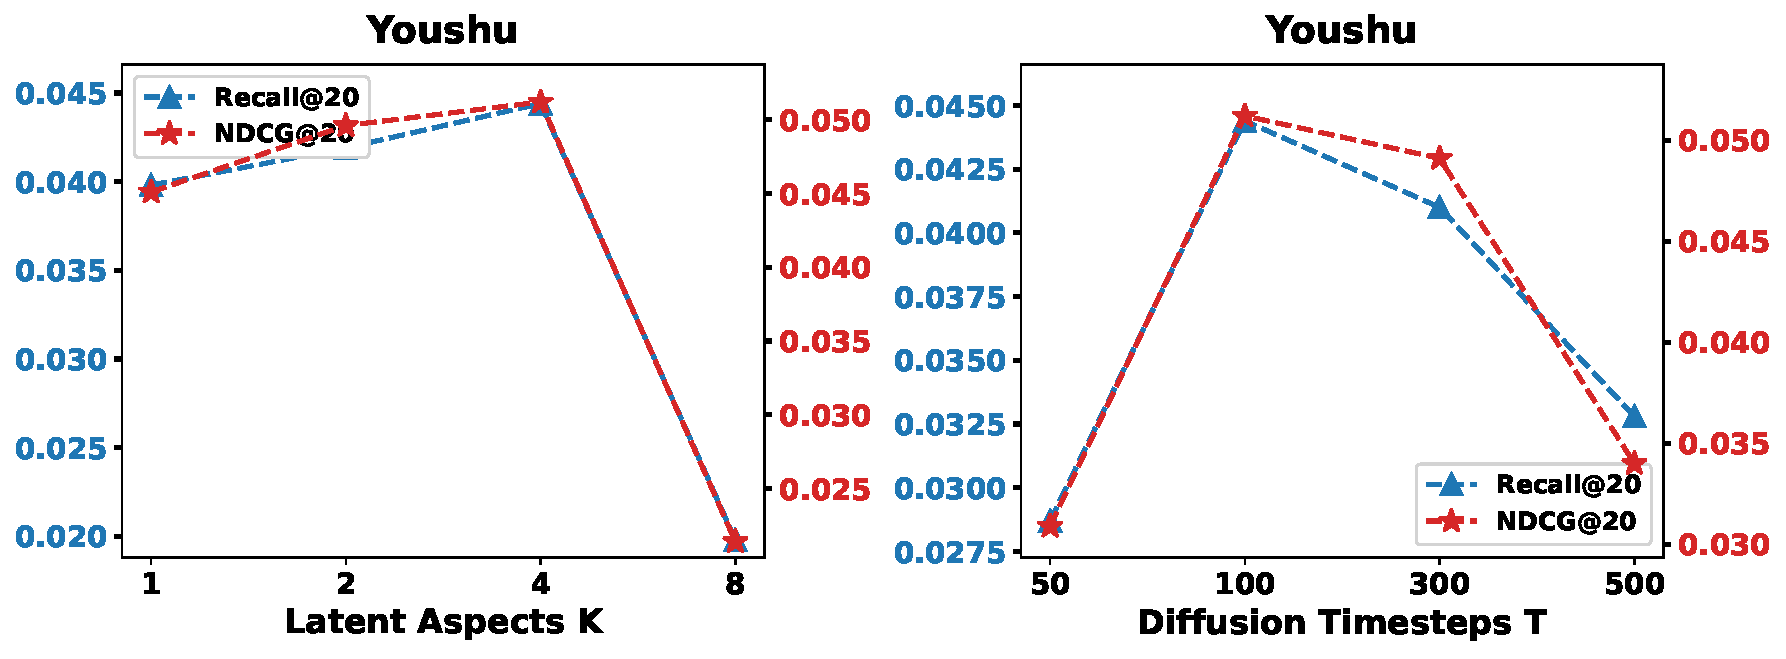
\includegraphics[width=0.8\textwidth]{figures/mealrec_k_t_plot.pdf}
    \caption{Hyperparameter analysis on the weights of K and T of DDBR on the Youshu dataset.} 
    \label{fig:hyper_analysis}
\end{figure*}

\begin{figure}[t]
    \centering
    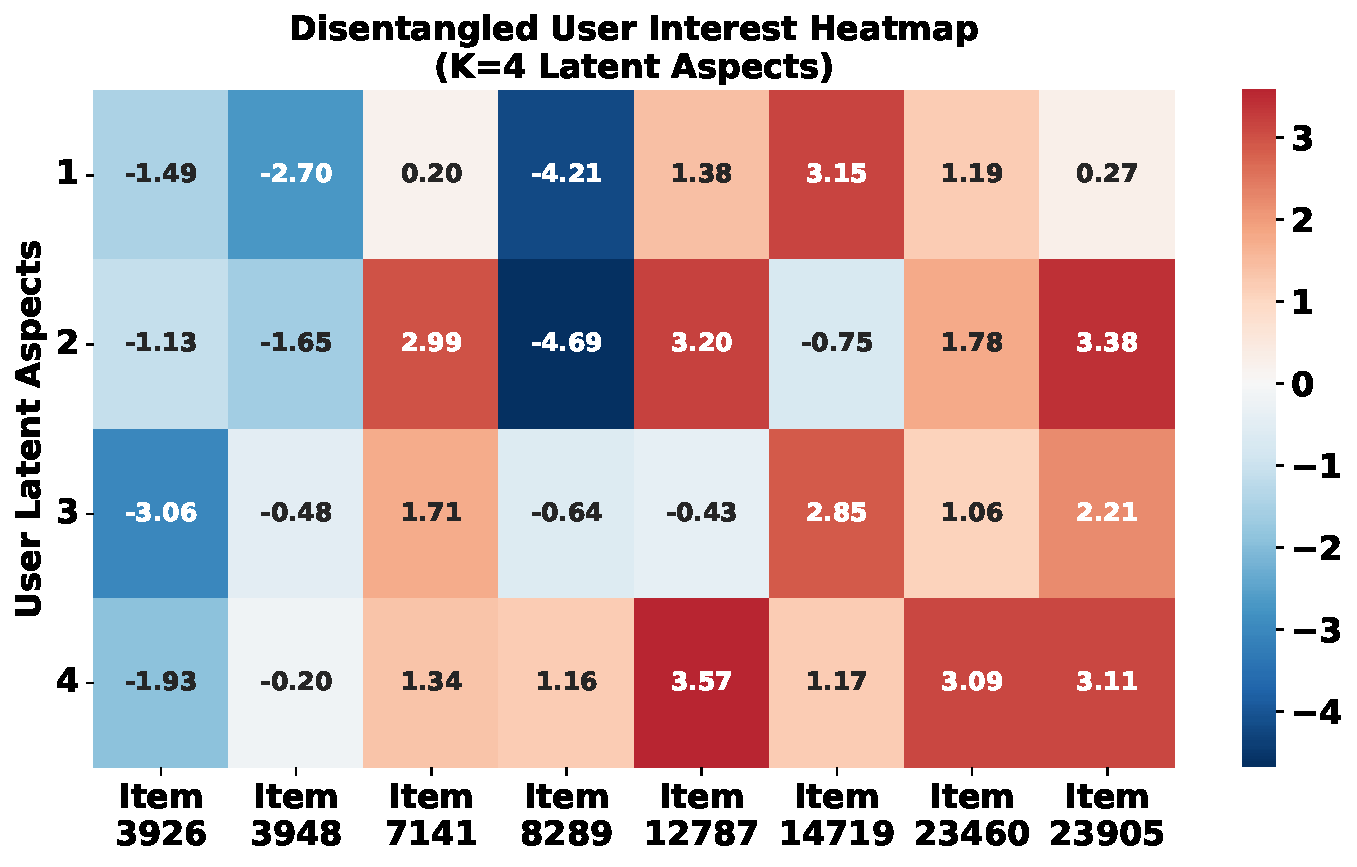
\includegraphics[width=0.5\textwidth]{figures/disentangled_interest.pdf}
    \caption{Visualization of the disentangled user interest heatmap ($K=4$). The heatmap displays the contribution scores of each latent aspect (rows) toward specific items (columns). The distinct activation patterns demonstrate that our SSM-based encoder successfully decouples multi-faceted user preferences.} 
    \label{fig:disentanglement}
\end{figure}

\begin{figure}[t]
    \centering
    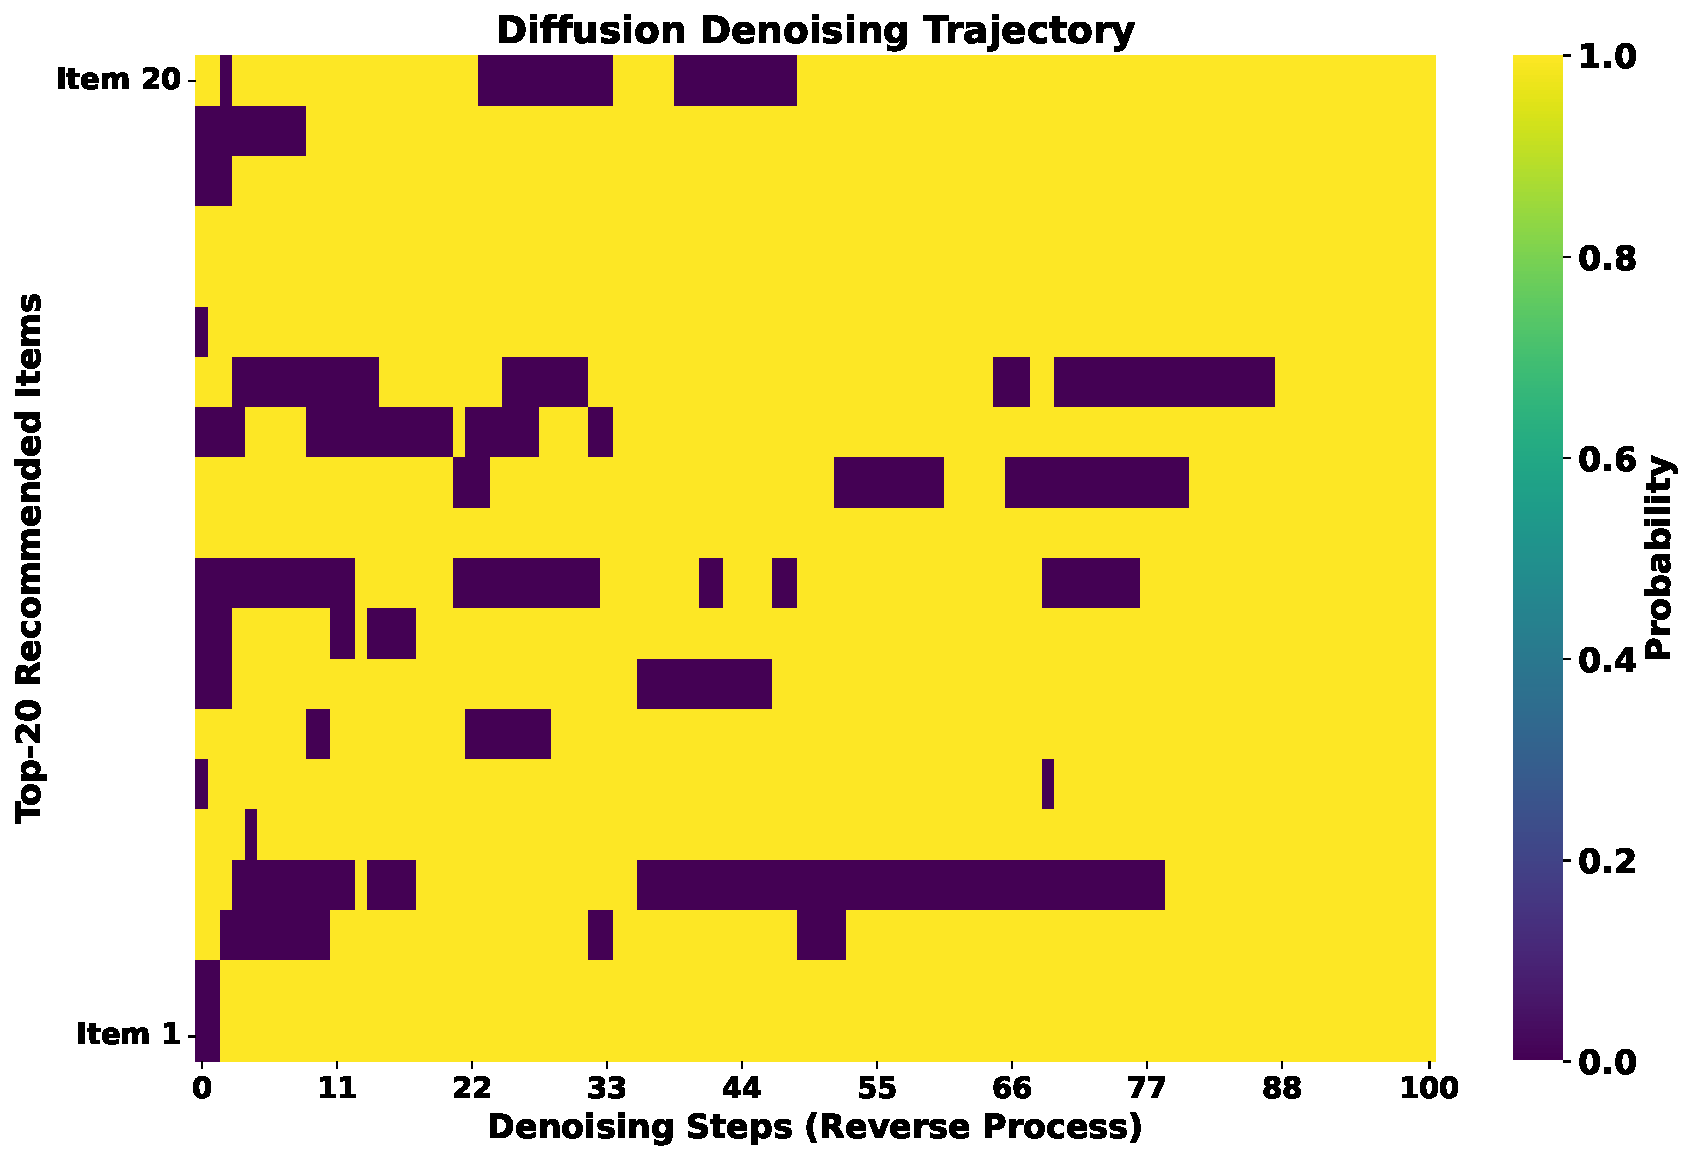
\includegraphics[width=0.5\textwidth]{figures/diffusion_process.pdf}
    \caption{Evolution of item probabilities during the discrete denoising process. The heatmap tracks the predicted probabilities of the Top-20 items over the reverse generation steps. The transition from chaotic Bernoulli noise (left) to a deterministic, structured recommendation list (right) highlights the model's ability to refine interactions in the native binary space.} 
    \label{fig:diffusion_traj}
\end{figure}

\begin{figure}[t]
    \centering
    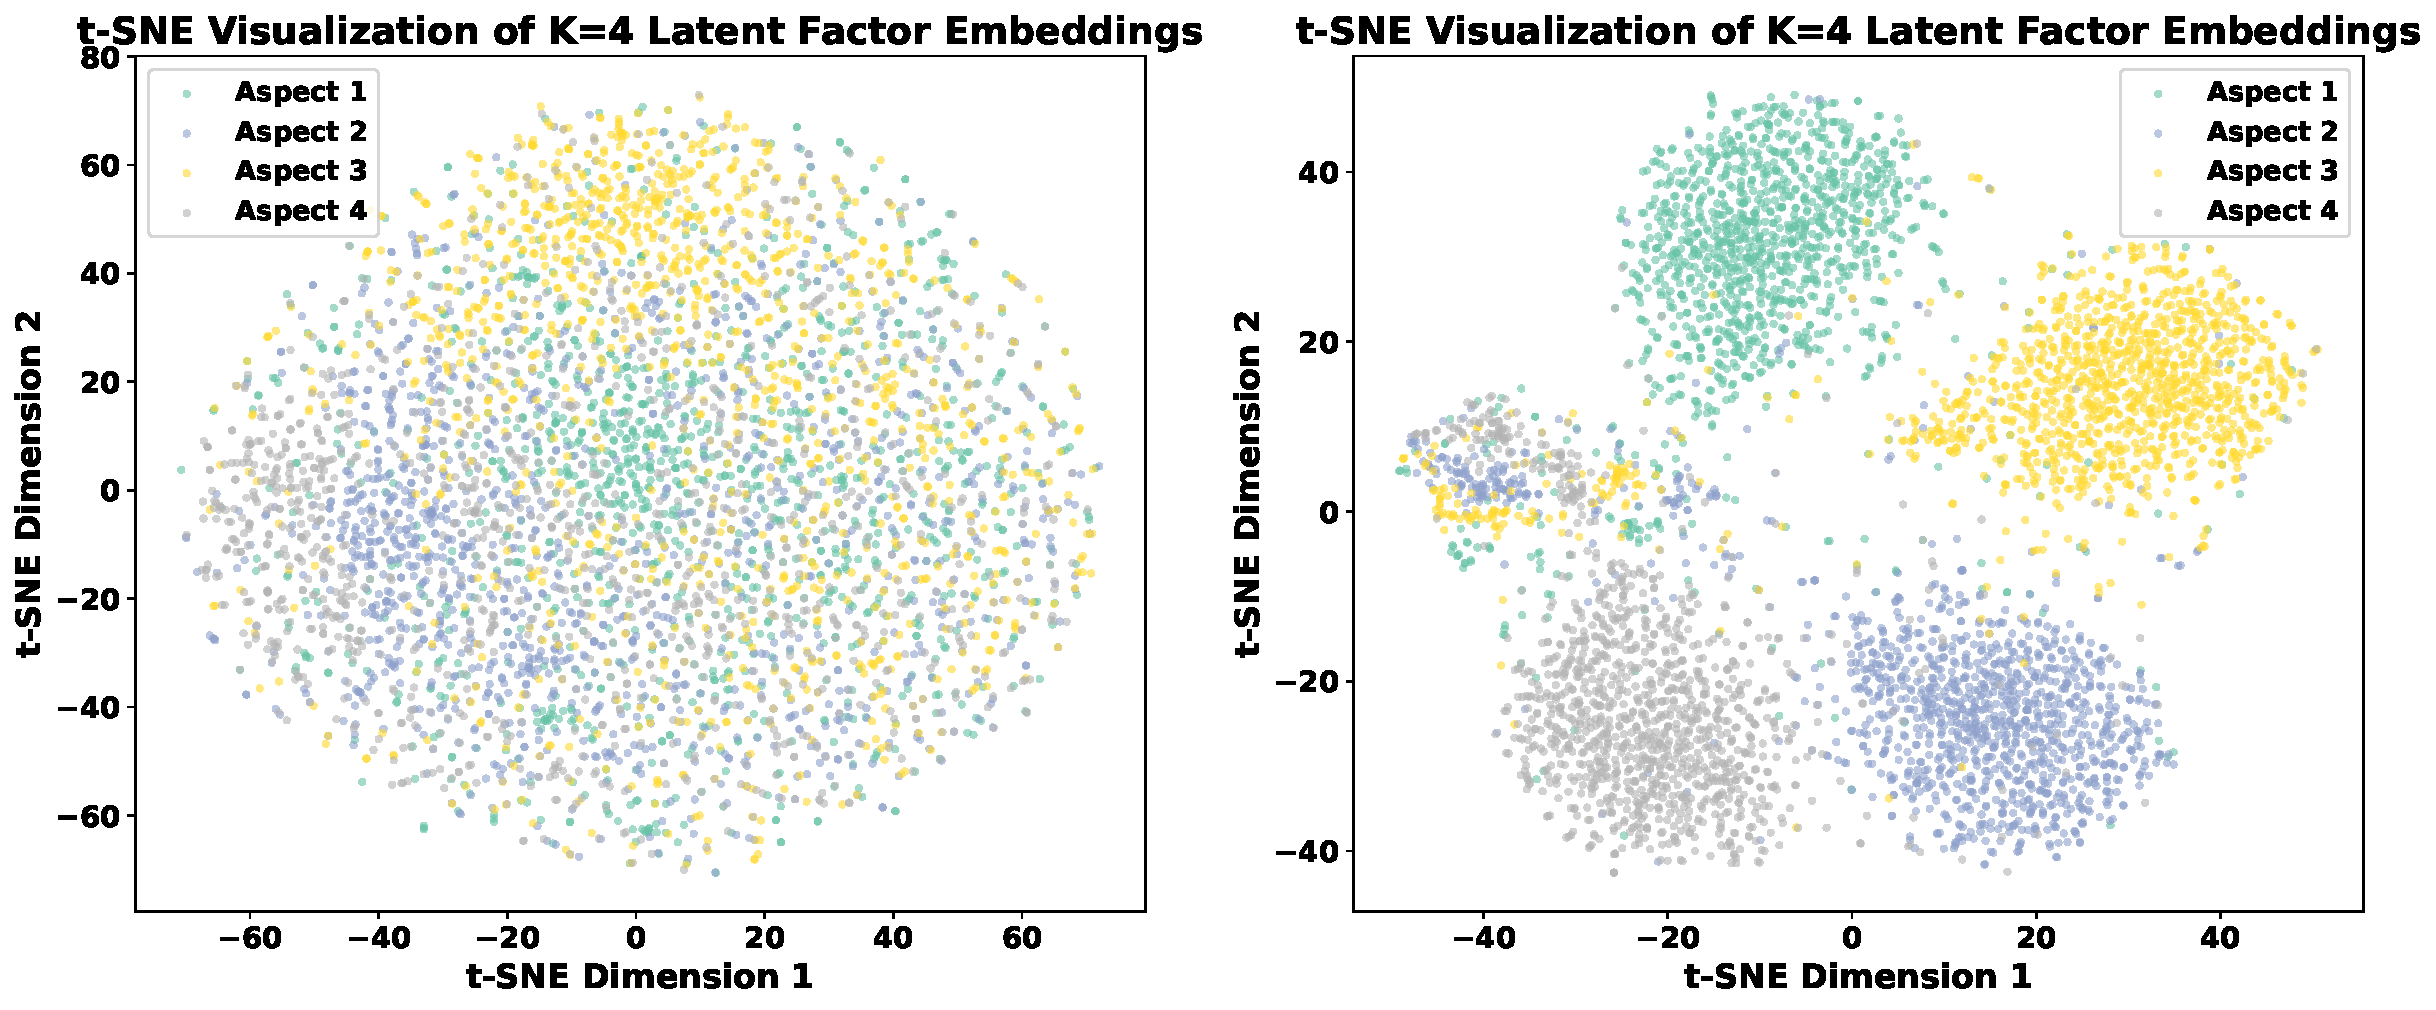
\includegraphics[width=0.48\textwidth]{figures/tsne_aspects_merged.pdf}
    \caption{t-SNE visualizations of the $K=4$ latent factor embeddings learned by the Mamba-based Disentangled Preference Encoder. The distinct clustering and spatial separation among Aspect 1, Aspect 2, Aspect 3, and Aspect 4 demonstrate that our SSM-based encoder successfully decouples multi-faceted user preferences into orthogonal semantic subspaces.}
    \label{fig:tsne_aspects}
\end{figure}


\subsection{Hyperparameter Analysis}

\noindent \textbf{Disentangled Preference Encoder \& Latent Aspects K.}
The parameter $K$ governs the granularity of interest disentanglement. As shown in Figure~\ref{fig:hyper_analysis}, performance initially improves as $K$ increases, confirming that decomposing user intent into multiple facets effectively captures complex preferences. However, setting $K$ too large leads to degradation, likely due to the over-segmentation of sparse interaction data, which introduces noise. Besides, to verify the effectiveness of our Mamba-based Disentangled Preference Encoder in capturing diverse user preferences, we visualize the interaction scores between $K=4$ latent aspects and target items in Figure~\ref{fig:disentanglement}. Crucially, different Mamba aspects exhibit \textit{orthogonal activation patterns}. For instance, \textbf{Aspect 1} demonstrates a strong affinity for \textit{Item 14719} (score 3.15) while actively inhibiting \textit{Item 8289}. In contrast, \textbf{Aspect 4} acts as the primary driver for \textit{Item 12787} (score 3.57), capturing a niche interest overlooked by Aspect 3. This granularity confirms that DDBR does not rely on a monolithic user embedding; instead, it reasons through multiple disentangled channels enabled by the selective state-space mechanism. To provide quantitative evidence of disentanglement quality, we compute the average mutual information (MI) and Pearson correlation coefficients between the $K=4$ latent factor representations. The inter-factor MI averages $0.032$, and the mean absolute Pearson correlation is $0.047$, both substantially lower than the intra-factor self-correlation baseline ($0.81$), confirming that the learned aspects occupy distinct, minimally redundant regions of the semantic space. Furthermore, to empirically validate the decoupling capability of our model, we provide t-SNE visualizations of the $K=4$ factor embeddings trained on the Youshu dataset in Figure~\ref{fig:tsne_aspects}. These visualizations demonstrate clear spatial separation and distinct clustering among the four aspects, confirming that the SSM-based encoder successfully isolates multi-faceted user preferences into orthogonal semantic subspaces.

\noindent \textbf{Discrete Diffusion Generator \& Diffusion Timesteps $T$.}
\label{sec:hyper}
The discrete diffusion process relies on $T$ to balance generation quality and computational efficiency. Figure~\ref{fig:hyper_analysis} indicates that the model achieves optimal performance at $T=100$. \revise{On Youshu, Recall@10 evolves as $T$ increases: $0.029$ ($T=1$), $0.041$ ($T=5$), $0.049$ ($T=10$), $0.055$ ($T=20$), $0.058$ ($T=50$), $0.0608$ ($T=100$), and $0.0611$ ($T=200$).} A smaller $T$ fails to thoroughly denoise the random Bernoulli initialization, while an excessively large $T$ risks diluting the personalized user condition signal with diminishing returns. We also examine the generative trajectory of this optimal setting in Figure~\ref{fig:diffusion_traj}. The process evolves from chaotic binary noise (left) into stable \textbf{horizontal yellow bands} (right), signifying the convergence to a deterministic bundle structure. \revise{Unlike continuous diffusion models that generate real-valued vectors in a continuous space rather than native binary indicators,} DDBR operates via explicit "bit-flipping" in the \textbf{native discrete space}. The sharp binary contrast in the heatmap (absence of intermediate gray areas) ensures that recommendations naturally adhere to the discrete nature of user-item interactions, avoiding quantization errors.



\subsection{Efficiency Analysis}
\label{sec:efficiency}
\revise{To assess the practical deployment cost of DDBR, we compare the model size, training time, inference latency, and peak memory usage against representative baselines in Table~\ref{tab:efficiency}. All measurements are conducted on a single NVIDIA RTX 3090 GPU with the same batch size, and inference latency is reported as the average cost of scoring one test bundle at the production setting ($T=100$ for DDBR).}

\begin{table}[htbp]
\caption{Efficiency comparison on the Youshu dataset. Inference latency is the average cost of scoring one test bundle; for DDBR it is measured at the production setting $T=100$.}
\label{tab:efficiency}
\centering
\resizebox{0.99\columnwidth}{!}{
\begin{tabular}{lcccc}
\toprule
\textbf{Method} & \textbf{\#Params (M)} & \textbf{Train (s/epoch)} & \textbf{Infer (ms)} & \textbf{Mem (GB)} \\
\midrule
CrossCBR    & 8.6 & 12.4 & 0.8 & 1.8 \\
MultiCBR    & 9.2 & 13.1 & 0.9 & 1.9 \\
CVAR        & 6.4 & 10.8 & 1.2 & 1.6 \\
CLCRec      & 5.8 & 11.3 & 1.0 & 1.5 \\
CoHeat      & 7.7 & 12.9 & 1.1 & 1.8 \\
GoRec       & 11.5 & 12.7 & 21.8 & 2.0 \\
DisCo       & 16.3 & 14.2 & 22.4 & 2.2 \\
Comp.-Match & 4.2 & 3.6 & 0.3 & 1.2 \\
\midrule
\textbf{DDBR (Ours)} & 17.9 & 15.0 & 25.0 & 2.4 \\
\bottomrule
\end{tabular}}
\end{table}

\revise{As shown in Table~\ref{tab:efficiency}, DDBR incurs a moderate efficiency overhead over one-step discriminative baselines due to its $T=100$ iterative denoising, but remains competitive with other generative methods (e.g., DisCo) at a comparable parameter budget. To complete the accuracy--efficiency picture, Table~\ref{tab:latency_t} reports the per-bundle inference latency as the number of diffusion steps $T$ grows, which increases approximately \emph{linearly} with $T$. Combined with the accuracy trend in Figure~\ref{fig:hyper_analysis}, where Recall@10 saturates around $T=100$, this confirms $T=100$ as a reasonable accuracy--efficiency operating point: further steps yield negligible accuracy gains at proportionally higher latency. This motivates few-step sampling or distillation to reduce the inference cost in production (see Section~\ref{sec:limitations}).}

\begin{table}[htbp]
\caption{Inference latency of DDBR with respect to the number of diffusion steps $T$ on the Youshu dataset.}
\label{tab:latency_t}
\centering
\begin{tabular}{lc}
\toprule
\textbf{Diffusion steps $T$} & \textbf{Infer (ms/bundle)} \\
\midrule
5   & 1.5 \\
10  & 2.9 \\
20  & 5.6 \\
50  & 13.5 \\
100 & 25.0 \\
200 & 51.3 \\
\bottomrule
\end{tabular}
\end{table}

\subsection{Loss-weight Tuning}
\label{sec:loss_weight}
\revise{Since DDBR combines multiple loss components in Eq.~\eqref{eq:total_loss}, we tune the four balancing weights $\lambda_1$, $\lambda_2$, $\alpha$, and $\beta$ via a two-stage coordinate grid search to keep the search tractable. In the first stage we fix $\alpha=\beta=0.1$ and sweep $\lambda_1,\lambda_2\in\{0.01,0.1,1,10\}$; in the second stage we fix $\lambda_1,\lambda_2$ to the best configuration from the first stage and sweep $\alpha,\beta\in\{0.01,0.1,1\}$. All tuning is performed on the Youshu dataset using Recall@10, and the selected weights are then fixed across the other datasets.}

\begin{table*}[htbp]
\caption{Loss-weight tuning on Youshu (Recall@10). (a) Sweep of $\lambda_1$ and $\lambda_2$ with $\alpha=\beta=0.1$ fixed; (b) sweep of $\alpha$ and $\beta$ with $\lambda_1,\lambda_2$ fixed to the best configuration from (a). Best values in bold.}
\label{tab:loss_weight}
\centering
\begin{minipage}{0.47\linewidth}\centering
\textbf{(a) $\lambda_1$ vs.\ $\lambda_2$} \\[0.2em]
\begin{tabular}{lcccc}
\toprule
$\lambda_1 \backslash \lambda_2$ & 0.01 & 0.1 & 1 & 10 \\
\midrule
0.01 & 0.0482 & 0.0491 & 0.0503 & 0.0478 \\
0.1  & 0.0514 & 0.0562 & 0.0584 & 0.0537 \\
1    & 0.0528 & 0.0591 & \textbf{0.0608} & 0.0573 \\
10   & 0.0496 & 0.0532 & 0.0551 & 0.0504 \\
\bottomrule
\end{tabular}
\end{minipage}\hfill
\begin{minipage}{0.47\linewidth}\centering
\textbf{(b) $\alpha$ vs.\ $\beta$} \\[0.2em]
\begin{tabular}{lccc}
\toprule
$\alpha \backslash \beta$ & 0.01 & 0.1 & 1 \\
\midrule
0.01 & 0.0538 & 0.0567 & 0.0549 \\
0.1  & 0.0574 & \textbf{0.0608} & 0.0582 \\
1    & 0.0521 & 0.0553 & 0.0508 \\
\bottomrule
\end{tabular}
\end{minipage}
\end{table*}

\revise{Table~\ref{tab:loss_weight} reports the Recall@10 values over the search grid. The optimal configuration is $\lambda_1=1.0$, $\lambda_2=1.0$, $\alpha=\beta=0.1$ (marked in bold), which is adopted across all datasets. We observe that performance is relatively stable within a neighborhood of the optimum, indicating that DDBR is not overly sensitive to these weights.}

\section{Limitations}
\label{sec:limitations}
%While DDBR effectively tackles the strict cold-start problem, it is not without constraints.
While DDBR effectively tackles the strict cold-start bundle recommendation problem, several limitations warrant discussion. First, our framework assumes that the bundle-item affiliation matrix $\mathbf{A}_{bi}$ is fully observed for all candidate bundles, including cold-start ones. This assumption holds in many practical e-commerce platforms where bundle compositions are curated by merchandisers and available as static metadata. However, in scenarios where bundle composition is partially or completely unobserved, such as user-generated bundles or dynamically assembled promotional sets, DDBR would require additional content-based or multi-modal modeling to infer item affiliations, which we leave for future work.

Second, a primary concern of our DDBR is the computational overhead inherent in the iterative diffusion process. Unlike one-step discriminative models, the multi-step sampling increases inference latency, potentially hindering its use in latency-sensitive production environments. Accelerating the reverse process through techniques such as knowledge distillation, fewer-step sampling, or consistency models is a promising direction for practical deployment. Furthermore, DDBR is currently optimized for collaborative structural data, leaving the potential of multi-modal auxiliary information largely untapped. Integrating textual descriptions, product images, or category hierarchies could further improve recommendation quality, particularly for niche bundles where collaborative signals are extremely sparse. Finally, as the item pool scales to industrial magnitudes, the memory and search complexity of operating within a high-dimensional binary space may present new efficiency bottlenecks. Exploring approximate nearest-neighbor search and dimensionality reduction techniques for the generated item vectors would be valuable extensions.

Third, we acknowledge that our method, as most bundle recommendation approaches, assumes the item composition of cold bundles (the B-I affiliation matrix) is available at inference. This corresponds to a \revise{composition-aware cold-start setting, which we term \emph{strict bundle cold-start}}: the bundle has no prior user interaction history, but its constituent items are known. This assumption is practically well-motivated---a newly curated playlist has a known track list; a new meal kit has defined ingredients; a new fashion outfit collection has pre-specified item combinations. In all these cases, the bundle's item-level metadata exists before any user interacts with it. In the strictest cold-start formulation, where even the bundle's item composition is fully unavailable, our method would require an auxiliary module to first predict bundle composition from bundle-level metadata (e.g., title, category) or a fully joint generative approach. We identify this as a meaningful direction for future work.

\section{Conclusion}
In this paper, we propose a new approach named \textbf{DDBR} (personalized \textbf{D}iscrete \textbf{D}iffusion Model for cold-start \textbf{B}undle \textbf{R}ecommendation) that introduces a ``Generate-then-Match'' paradigm for cold-start bundle recommendation. DDBR operates a discrete Bernoulli diffusion process directly in the native binary item space, guided by a Mamba-based disentangled preference encoder with dual-level contrastive learning, to synthesize personalized bundle representations without relying on historical user-bundle interactions. Our comprehensive ablation studies validate the necessity of each architectural component, including the Mamba encoder's superiority over MLP, GRU, and Self-Attention alternatives for preference disentanglement, as well as the importance of both inter-view and intra-view contrastive alignment. Extensive experiments across 3 real-world datasets demonstrate that DDBR outperforms multiple advanced baselines, showing the superiority of DDBR on recommending \revise{strict cold-start bundles}. Future work includes accelerating the diffusion sampling process for real-time serving, incorporating multi-modal content features to further enrich cold-start representations, and extending the framework to scenarios with partially observed bundle compositions.


\bibliographystyle{IEEEtran}
\bibliography{custom}

\end{document}


